\documentclass[a4paper,11pt]{article}
\usepackage{amsmath}
\usepackage[authoryear,round]{natbib}
\usepackage{longtable}
\usepackage{threeparttable}
\usepackage{array}
\usepackage{hyperref}
\usepackage{geometry}
\usepackage{graphicx}

\usepackage{etoolbox}
\preto\tabular{\setcounter{magicrownumbers}{0}}
\newcounter{magicrownumbers}
\newcommand\rownumber{\stepcounter{magicrownumbers}\arabic{magicrownumbers}}

\usepackage{pdflscape}
\geometry{verbose,a4paper,tmargin=26mm,bmargin=26mm,lmargin=28mm,rmargin=28mm}

\usepackage[singlelinecheck=off]{caption}


\usepackage[latin1]{inputenc}




\title{Benchmarking ADaCGH2 and comparison with previous versions}
\author{Ramon Diaz-Uriarte$^{1}$}






\begin{document}
\maketitle

\begin{center}
1. Department of Biochemistry,
Universidad Autonoma de Madrid
Instituto de Investigaciones Biomedicas ``Alberto Sols'' (UAM-CSIC), Madrid
(SPAIN).
{\tt rdiaz02@gmail.com}
\end{center}

\tableofcontents
\listoftables
\listoffigures



\clearpage

\section{Introduction}
We provide here comparisons with the former version of ADaCGH2 (v.\ 1.10,
as available in BioConductor v.\ 2.12) as well as some comparisons against
non-parallelized executions and, finally, some details about recommended
patterns of usage. The benchmarks shown here total over more than 1640 hours
of wall time (about 70 days).
Before showing the results, we provide information
about the hardware and data sets.



\subsection{Data set and hardware}
\label{sec:data-set-hardware}

We will use a simulated data set that contains 6,067,433 rows and up to
4000 columns of data; these are, thus, data for an array with 6 million
probes and data for up to 4000 subjects. Many of the examples shown below
will use smaller subsets of the data, smaller in terms of the number of
subjects or samples (columns). There are 421,000 missing values per data
column. 

To give an idea of sizes, the ASCII file with the data for the 1000 column
data is about 96 GB\footnote{All sizes are computed from the reported size
  in bytes or megabytes, using 1024, or powers of 1024, as denominator.},
and an archived set of 2000 columns, compressed with bzip2, occupies 72
GB. The RData for those same data (1000 columns) is 46 GB (without
compression; 41 GB with the standard R compression); in a freshly started
R session, loading the RData will use 46 GB (as reported by
\texttt{gc()}). The RData object with the 1000 columns, when loaded into R
in the PowerEdges, takes 13 minutes to load and uses a total of about 46
GB (45.7 from calls to \texttt{gc} before and after loading the object,
and adding Ncells and Vcells, or 45.6 as reported by
\texttt{object.size}). Note that this is not the result of the object
being a data frame and having a column with identifiers (a factor),
instead of being a matrix; a similarly sized matrix with just the numeric
data for the probes (i.e., without the first three columns of ID,
chromosome, and location) has a size of 45.2 GB (therefore, the difference
of 300 MB due to the first column, ID, being a factor with the
identifiers, is minute relative to the size of the matrix).  As a
reference for the size of the data set,







 %%             used    (Mb) gc trigger    (Mb)   max used    (Mb)
 %% Ncells    6272458   335.0    9532693   509.2    6273371   335.1
 %% Vcells 6102207940 46556.2 6634368466 50616.3 6102370100 46557.4 









The examples below were run on a Dell PowerEdge C6145 chasis with two
nodes. Each node has 4 AMD Opteron 6276 processors; since each processor
has 16 cores, each node has 64 cores. One node has 256 GB RAM and the
other 384 GB of RAM. Both nodes are connected by Infiniband (40Gb/s).  For
the data presented here, when using a single node, the data live on an xfs
partition of a RAID0 array of SAS disks (15000 rpm) that are local to the
node doing the computations. When using the two nodes, the data live on
that same local SAS drive, which is seen by the other node using a simple
NFS setup (we have also used distributed file systems, such as FhGFS, but
they have tended to be a lot slower in these experiments; your mileage
might vary). Therefore, in the table entries below, executions using both
nodes will indicate ``124 cores'' \footnote{124 is not a typo; it is 124,
  even if the total number of cores is $128 = 64 * 2$. This is due to the
  following documented issue with Open MPI and Infiniband:
  \url{http://www.open-mpi.org/community/lists/users/2011/07/17003.php},
  and since $128^2 = 16384$, we are hitting the limit, and we have not had
  a chance to correct this problem yet. Regardless, the penalty we would
  pay would be a difference of 4 process out of 124.}

  
We will also show some examples run on an HP Z800 workstation, with 2
Intel Xeon E5645 processors (each processor has six cores), and 64 GB of
RAM. The data live on an ext4 partition on a SATA disk (7200 rmp). % In the


In both systems, the operating system is Debian GNU/Linux (a mixture of
Debian testing and Debian unstable). The Dell PowerEdge nodes were running
version R-2.15.1 as available from the Debian repository (v.\ 2.15.1-5)
or, later, R-3.0.1, patched (different releases, as available through May
and June of 2013), and compiled from sources. The Xeon workstation was
running R-2.15.1, patched version (2012-10-02 r60861), compiled from
sources or, later R-3.0.1, patched (different releases, as available
through May and June of 2013). Open MPI is version 1.4.3-2 (as available
from Debian).


\subsection{Tables: column name explanation}
For the tables below, the meaning of columns is as follows:

\begin{description}

\item[Wall time (min.)] The ``elapsed'' entry returned by the command
  \texttt{system.time}. This is the real elapsed time, the wall time, in
  minutes, since the function was called.
  
  It is important to understand that these timings can be variable. In
  many cases, we show repeated executions with the exact same settings,
  that will help show the variability in those numbers.

\item[Memory (GB)] The memory used by the master R process. This is the
  sum of the two rows of the ``max used'' column reported by
  \texttt{gc()}, in R, at the end of the execution of the given
  function. This number cannot reflect all the memory used by the function
  if the function spawns other R processes. 

\item[$\Sigma$ Memory (GB)] A simple attempt to measure the memory used by
  all the processes\footnote{Just adding the entries given by \texttt{top}
    or \texttt{ps} will not do, and will overestimate, sometimes by a huge
    amount, the total memory used.}. Right before starting the execution
  of our function, we call the operating system command \texttt{free} and
  record the value reported by the ``-/+ buffers/cache'' row. Then, while
  the function is executing, we record, every 0.1 seconds (or every 0.05
  seconds), that same quantity. The largest difference between the
  successive measures and the original one is the largest RAM
  consumption. Note that this is an approximation. First, if other process
  start executing, they will lead to an overestimation of RAM usage; this,
  however, is unlikely to have had serious effects (the systems were
  basically idle, except for light weight cron jobs), though a few results
  in the tables suggest this happened in a few instances (related to
  backup processes). Second, sampling is carried out every 0.5 seconds, so
  we could miss short peaks in RAM usage but, again, this is unlikely to
  lead to a serious underestimation.
  % (at least one likely example of such underestimation shows in the
  % tables below)
  % . Finally, the coherence of repeated executions and the clear patterns
  % both within and among machines suggests that this procedure captures the
  % key
  
  \item[Columns] The number of data columns of the data set.
  \item[Method] The analysis method. ``Haar'' for HaarSeg, ``CBS'' for
    Circular Binary Segmentation (from package \texttt{DNAcopy}), ``HMM''
    for the HMM approach in package \texttt{aCGH}, ``BioHMM'' for the
    non-homogeneous HMM method in package \texttt{snapCGH}, and ``GLAD''
    for the method with the same name in package \texttt{GLAD}. See 
    section \ref{methodproblems} for why other methods are not shown in
    the tables.


  \item[MPI/Fork] Whether forking (via \texttt{mclapply}) or MPI (using
    the facilities provided by package \textbf{Rmpi}, which are called
    from package \textbf{snow}) are used to parallelize execution.

    The ``NP'' entries in table \ref{nonparall} refer to non-parallelized
    execution, using the original packages\footnote{The packages are
      DNAcopy, as available from BioConductor, and the HaarSeg package,
      available from R-forge:
      \url{https://r-forge.r-project.org/projects/haarseg/}}.

    The entries marked as ``-LB'' correspond to the load-balanced options
    with the new version of ADaCGH2 (setting \texttt{loadBalance = TRUE},
    in v.\ $\ge 2.3.4$).


\item[Cores] Number of cores used. In most cases, when running in the AMD Opteron
  machines we used all 64 cores, and when running on the Intel Xeon
  machine we used all 12 cores, but not always. When running over both AMD
  Opterons we used 124 cores (see above).

\item[Procs.\ per node] When using MPI, the total number of R processes
  that can run in a node; this is the parameter \texttt{npernode} passed
  to \texttt{mpirun} (from Open MPI). When running on a single node, that
  is the number of R slaves + 1.
\item[Universe size] The number of slave nodes in the MPI universe (over
  all nodes in the universe). This is the parameter \texttt{count} passed
  to \texttt{makeMPIcluster} in R.

\item[Version] The version of ADaCGH2. For simplicity, ``Old'' means
  version 1.10 and ``New'' versions 2.1 and larger.
  
  The post-fix ``-noNA'' means the new version was run using option
  \texttt{certain\_noNA = TRUE}; note that the old version of ADaCGH2
  assumes there are no missing values in the data. Thus,
  \texttt{certain\_noNA = TRUE} is the closest to what the old version assumes. 

\item[ff/RAM] Where applicable in the tables, if the data for the analysis
  had been stored as an \textit{ff} object, or as a data frame inside an
  RData that was loaded before the analysis.
  

\end{description}




\section{Comparison with v.\ 1.10 of ADaCGH2}

\subsection{Main differences between the old (v.\ 1.10) and new versions
  (v.\ $\ge$ 2.1.3) of ADaCGH2}


The code for the new version of ADaCGH2 represent a major rewrite of most
of the code in the former version. Listed here are some of the major
advantages of the new version; they are shown in approximately decreasing
order of importance from the user's point of view.


\begin{description}

\item[Reading of large data sets] The new version of ADaCGH2 can read data
  sets much larger than the old one (see section \ref{comp-read}). In a
  machine with 64 GB RAM the old version cannot read data sets with 500
  columns (each with 6 million probes), whereas data sets with 4000
  columns can be read with the new version (see table \ref{read-coleonyx})
  and the scaling of the memory consumption with number of columns
  suggests that much larger data sets could be read. Likewise, in machines
  with 256 and 384 GB of RAM (tables \ref{read-gallotia} and
  \ref{read-lacerta}) data sets of 2000 columns could not be read with the
  old version of ADaCGH2, but data sets of 4000 columns are read with the
  new version and, again, the scaling of memory consumption with number of
  columns suggests (see Figure \ref{fig-read}) that much larger data sets could be
  read and, even for the sizes of data that can be read by the old
  version, reading is faster with the new version because it can make much
  better usage of available hardware (RAID arrays for disks).



\item[Missing value handling] The old version of ADaCGH2 used row-wise
  deletion of missing values when reading data: a probe would be deleted
  from the data if it had one missing value over all subjects. Analysis
  could be speed up, as no checks or provisions had to be taken for
  dealing with NAs, and all procedures are simplified, as the data are
  then known to be complete. However, row-wise deletion of missing values
  is probably not an appropriate approach, especially as the number of
  samples increases (because the probability that a given probe will then
  be left out of the analysis increases). The new version of ADaCGH2 deals
  with missing values column by column, so for each column (or subject)
  all available data (or probes) are used in the
  segmentation. Nevertheless, the new version incorporates a setting to
  provide speed ups when the user is certain that there are no missing
  values (\texttt{certain\_noNA = TRUE}).


\item[Analysis of large data sets] The old version of ADaCGH2 cannot
  analyze large data sets, as it cannot read them and it cannot use data
  read by the new version since the old version assumes there are no
  missing values in the data after reading.


\item[Forking] The new version of ADaCGH2 allows for the usage of forking
  to parallelize reading and analysis. In Unix-based environments
  (including Unix, GNU/Linux, and Mac OS), forking can be faster, less
  memory consuming, and much easier to use than using an explicit cluster.


\item[Speed] The new version is generally slightly faster than the old one
  for the default options (load balancing and forking). Further speed
  improvements can be achieved in some cases, for instance by not using
  load balancing with certain methods (e.g., HaarSeg); see details in
  section \ref{comp-anal}.


\item[Flexibility of reading data] The new version of ADaCGH2 has not
  removed the mechanisms of reading data available in the old
  version. Thus, when data are small or memory is plentiful, reading data
  from a single RData is an available option. But the new version adds new
  mechanisms, mainly reading from a text file and from a directory of
  text files, that, as discussed, allow for reading much larger data sets.

\item[Usage of data read from the other version] The new version of
  ADaCGH2 can accept data read by the old version. However, the old
  version of ADaCGH2 cannot accept data from read by the new version
  unless the original data contained no missing values at all: the old
  version of ADaCGH2 assumes that data that have been read contain no
  missing values.


\item[Flexibility of analysis options] The new version allows gives the
  user more options for analysis, which can help adapt analysis to
  available hardware, therefore resulting in faster speed and/or decreased
  memory consumption. In particular, the user can choose to use MPI or
  forking (option \texttt{typeParall} in the segmentation and plotting
  functions) and to use, or not, load balancing (options
  \texttt{loadBalance} to segmentation and plotting functions).

\item[Dependencies] The old version depends on package \texttt{snowfall}
  for parallelization, whereas the new depends only on
  \texttt{multicore}. This makes the new version less likely to break in
  the future, as \texttt{multicore} is one of the core packages
  distributed with R (whereas, for instance, there were some problems with
  \texttt{snowfall} immediately following the release of v.\ 3 of R).

  % In addition, snowfall is difficult to use with Open MPI, probably the
  % most widely used approach for MPI, and often the recommended one for R.


\item[More flexible options for load balancing] The old version of ADaCGH2
  forced load balancing. Whether or not load-balancing is the best
  approach depends on the size and number of jobs relative to the number
  of cores. As shown in the tables (see tables \ref{anal-coleonyx},
  \ref{anal-lacerta}, \ref{anal-gallotia}), not using load balancing can
  sometimes lead to speed improvements. The new version of ADaCGH2 allows
  not to use load balancing with the argument \texttt{loadBalance = FALSE}.


\item[Limiting RAM consumption] Limiting RAM usage during reading and
  analysis is simple with the new version of ADaCGH2: limit the number of
  processes that are allowed to run simultaneously. This is not possible
  with the old version of ADaCGH2.

\item[Method availability] Two of the methods available, HMM and BioHMM,
  depend on packages \texttt{aCGH} and \texttt{snapCGH}. These two
  packages haven been updated since 2010 and 2009, respectively, and aCGH
  will no longer be maintained (personal communication from the
  authors). There is code in ADaCGH2 (including both C and R code), taken
  and modified from those packages, that can be readily uncommented to
  make these two methods available in ADaCGH2 if either of those packages
  were not to pass checks in future versions of BioConductor.
 
\end{description}






\subsection{Segmentation methods used}\label{methodproblems}

The methods available in ADaCGH2 are (see further details in the help of
function \texttt{pSegment}):

\begin{itemize}

\item HMM, as described by \cite{hmm-fridlyand} and implemented in package
  \cite{aCGHpackage}. 

\item BioHMM, a non-homogeneous HMM, described in \cite{biohmm} and
  implemented in package \cite{snapCGH}. 

\item A wavelet-based method, proposed in \cite{waves-hsu}. This is called
  \texttt{pSegementWavelets} in ADaCGH2. 

\item Another wavelet-based method, HaarSeg, published in
  \cite{haarseg-paper}. This was later made available as an R-package as
  \cite{haar-package}.

\item The CGHseg method described in \cite{cghseg}. An implementation of
  \textbf{part} of this method is available in the R package
  \cite{tilingarray}, but ADaCGH2 is the first R implementation of the
  full description of the CGHseg procedure (see comments in the help of
  function \texttt{pSegmentCGHseg}).

\item The popular Circular Binary Segmentation approach, described in its
  current implementation in \cite{CBS-paper} and implemented in package
  \texttt{DNAcopy}.

\item GLAD, a method first described in \cite{glad-paper} and implemented
  in \cite{glad-package}.

\end{itemize}


The tables below only show benchmarks for methods HMM, BioHMM, HaarSeg
(referred as Haar) and CBS. CGHseg and the wavelet approach described in
\cite{waves-hsu} cannot be when any chromosome has a large number of
probes because of their memory use. With CGHseg the problem arises in the
underlying \texttt{tilingArray} package, in the internal step of computing
the ``costMatrix'', a function called by the function \texttt{segment} in
\texttt{tilingArray}.  When analyzing the first chromosome (for a single
subject), the request is for 1493 GB.  For the wavelet approach, the
problem shows up in the clustering step, when function \texttt{pam} (from
package \texttt{cluster}) is called. For instance, the memory requirements
for a chromosome of 350000 probes would exceeded 400 GB (the request is
for a vector of doubles of size $1 + (n * (n - 1))$.  It must be
emphasized that, in both cases, it is not the complete 6 million probes,
nor using multiple subjects, which causes the problems: neither of the
methods is capable of analyzing the first chromosome for a single subject.
GLAD can deal with large data sets in terms of memory usage, but it
extremely slow. After more than four days, the method had not been able to
finish the analysis of the 50-column data set in the machines with 64
cores; on close inspection, the problem lies in function
\texttt{OptimBkpFindCluster}, a C function internal to the package, and is
not attributable, therefore, at the initial segmentation method.  Finally,
to run method BioHMM we often had to increase the \texttt{ulimit} (stack
limit), by using \texttt{ulimit -u}, from the shell.



\clearpage
\subsection{Reading data}\label{comp-read}

The next three tables show time and memory consumption when reading data
using the recommended approach with each version of the package. Some of
the major patterns and results are:

\begin{description}
\item[Size limits for old version] Table
\ref{read-coleonyx} \textbf{cannot} show reading benchmarks for the old
version with data sets of sizes 500, 1000, 2000, or 4000, as those could
not be read with the old version (R run out of memory). Likewise, tables
\ref{read-gallotia} and \ref{read-lacerta} show reading benchmarks for the
old version with up to 1000 columns, because the AMD Opteron machines with
$\ge$ 256 GB RAM could not read data sets of sizes 2000 or
4000, as R could not allocate the necessary memory.% \footnote{The details about how much memory can be
  % successfully requested by a single process depend on settings such as
  % the overcommit policy and the vm.overcommit_ratio and the RAM and swap
  % of the system and how much memory is already being used by other
  % processes. For the three systems used, the maximum memory that could be
  % requested, as shown in \texttt{CommitLimit} in \texttt{/proc/meminfo}
  % was 66050908 kB, 262878296 kB, and 395261068 kB, for Coleonyx, Gallotia,
  % and Lacerta. This numbers, when using a vm.overcommit setting of 2,
  % i.e., with overcommit disabled, are the same as those obtained from
  % vm.overcommit_ratio * RAM + swap. In all cases, the machines were under
  % very light load from other processes when running the benchmarks, and
  % thus R was not killed when requests were of about, or larger than, the
  % figures given above.}.

In contrast, the new version is capable of reading data sets of 4000
columns in all machines, without getting anywhere near the memory limits
of the machines. Moreover, the \textbf{scaling} (see also figure
\ref{fig-read}) shows that the total number of columns could be increased
to much larger number and, in addition, that the total memory used can be
limited by setting the number of cores used (of course, at the possible
expense of reduced speed ---but see next point): for instance, compare row
32 with 33, and row 34 with 35 in table \ref{read-coleonyx}; rows 41 to 44
in table \ref{read-gallotia}; and rows 30, 31, 32, 33 in table
\ref{read-lacerta}.


\item[Speed of new and old version] Reading speed differences are small
  (and likely of little consequence for users) for small sized data sets;
  reading is faster at all sizes with the new version in the most capable
  machines, but is faster with the old version in the Intel Xeon
  machine. However, as data sets grow larger in size, reading speeds are
  much faster with the new version than the old by factors of about 4x.

\item[Speed and number of cores in new version] Reading speed does not
  always increase with the number of cores. Look at rows 32 to 35 in table
  \ref{read-coleonyx}; rows 41 to 44 in table \ref{read-gallotia}; and
  rows 30 to 33 in table \ref{read-lacerta}. In particular, the number of
  spindles and the speed of the drives is likely to have a large effect on
  the benefits of parallelizing reading. In the Intel Xeon machine all the
  data are on an ext4 partition that lives on a single SATA hard drive,
  whereas in the AMD Opteron machines the data are on an xfs partition
  that is, physically, for each machine, on four 600 GB SAS disks
  configured as a RAID0 array. In addition, the reading step is generally
  faster the less full the partition is and the type of file system is
  also likely to affect.

  If the reading operation is to be performed many times, or an very large
  set of data, it would pay off to experiment with the number of cores
  used for reading, which can be done with the option \texttt{mc.cores} to
  the function \texttt{inputToADaCGH}.

\end{description}

\clearpage
\begin{figure}[h!]
\begin{center}
  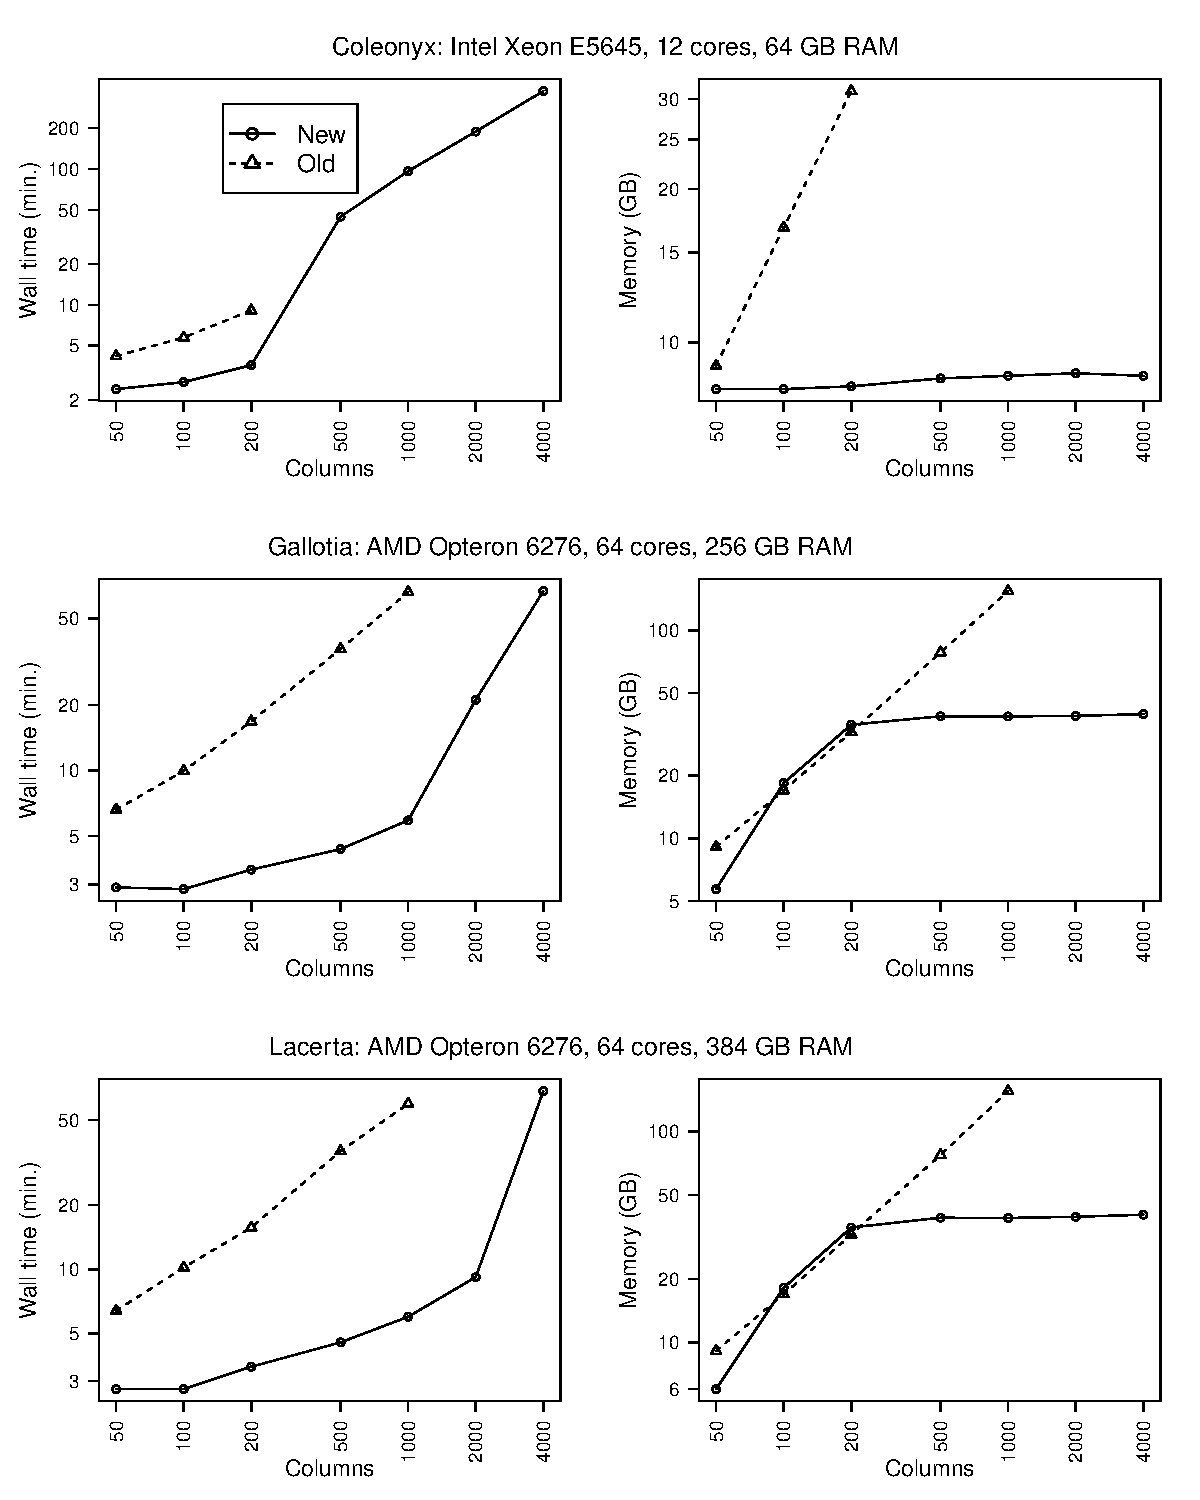
\includegraphics[width=16.1cm,keepaspectratio]{reading-benchmark-fig.pdf}
\end{center}
\caption[Wall time and memory usage when reading data: version
comparison]{\label{fig-read} Comparison between old and new versions in
  wall time and memory usage when reading data as a function of number of
  columns (samples). Both axis shown in log scale. The figure shows the
  default use cases: using 12 cores in the Intel Xeon machine and 64 cores
  in the AMD Opterons; note that better speeds (and lower memory usage)
  can be achieved by decreasing the number of cores used (see
  tables). When more than one benchmark is available for a scenario, the
  median is shown.}
\end{figure}

\begin{center}
% mylatex(tmp <- with(all.read, {     tmp2 <- all.read[all.read$machine == "Coleonyx", ]     cols <- c(1:4, 6, 5)     tmp4 <- with(tmp2, {         tmp3 <- tmp2[order(ncols, numcores, Version_ADaCGH2),              cols]         rownames(tmp3) <- 1:nrow(tmp3)         tmp3     })     attributes(tmp4)$mycolnames <- attributes(all.read)$mycolnames[cols]     tmp4 }), rowlabel = "", colheads = attributes(tmp)$mycolnames, longtable = TRUE,      lines.page = 900, caption = "Reading benchmarks for Coleonyx: Intel Xeon E5645, 12 cores, 64 GB RAM",      file = "read-coleonyx.tex") 
%

\setlongtables


\begin{longtable}{lrrrrrl}\caption{Reading benchmarks for Coleonyx: Intel Xeon E5645, 12 cores, 64 GB RAM} \tabularnewline
\hline\hline
\multicolumn{1}{l}{}&\multicolumn{1}{c}{Wall time (min.)}&\multicolumn{1}{c}{Memory (GB)}&\multicolumn{1}{c}{$\Sigma$ Memory (GB)}&\multicolumn{1}{c}{Columns}&\multicolumn{1}{c}{Cores}&\multicolumn{1}{c}{Version}\tabularnewline
\hline
\endfirsthead\caption[]{\em (Reading benchmarks for Coleonyx: Intel Xeon E5645, 12 cores, 64 GB RAM, continued)} \tabularnewline
\hline
\multicolumn{1}{l}{}&\multicolumn{1}{c}{Wall time (min.)}&\multicolumn{1}{c}{Memory (GB)}&\multicolumn{1}{c}{$\Sigma$ Memory (GB)}&\multicolumn{1}{c}{Columns}&\multicolumn{1}{c}{Cores}&\multicolumn{1}{c}{Version}\tabularnewline
\hline
\endhead
\hline
\endfoot
\label{read-coleonyx}
1&$  6.9$&$ 1.33$&$ 8.1$&$  50$&$12$&New\tabularnewline
2&$  2.3$&$ 1.33$&$ 7.8$&$  50$&$12$&New\tabularnewline
3&$  6.0$&$ 1.33$&$ 7.7$&$  50$&$12$&New\tabularnewline
4&$  6.0$&$ 1.33$&$ 8.1$&$  50$&$12$&New\tabularnewline
5&$  4.2$&$ 9.05$&$ 9.0$&$  50$&$$&Old\tabularnewline
6&$  4.6$&$ 9.05$&$ 8.9$&$  50$&$$&Old\tabularnewline
7&$  4.5$&$ 9.05$&$ 8.6$&$  50$&$$&Old\tabularnewline
8&$  4.2$&$ 9.05$&$ 9.0$&$  50$&$$&Old\tabularnewline
9&$  4.1$&$ 9.05$&$ 9.0$&$  50$&$$&Old\tabularnewline
10&$ 11.2$&$ 1.33$&$ 8.2$&$ 100$&$12$&New\tabularnewline
11&$  3.1$&$ 1.33$&$ 7.8$&$ 100$&$12$&New\tabularnewline
12&$ 10.2$&$ 1.33$&$ 8.3$&$ 100$&$12$&New\tabularnewline
13&$ 10.1$&$ 1.33$&$ 8.3$&$ 100$&$12$&New\tabularnewline
14&$  7.1$&$16.93$&$17.0$&$ 100$&$$&Old\tabularnewline
15&$  5.9$&$16.93$&$16.4$&$ 100$&$$&Old\tabularnewline
16&$  5.5$&$16.93$&$16.6$&$ 100$&$$&Old\tabularnewline
17&$  5.6$&$16.93$&$17.0$&$ 100$&$$&Old\tabularnewline
18&$ 21.8$&$ 1.33$&$ 8.4$&$ 200$&$12$&New\tabularnewline
19&$ 17.4$&$ 1.33$&$ 8.0$&$ 200$&$12$&New\tabularnewline
20&$ 17.9$&$ 1.33$&$ 8.0$&$ 200$&$12$&New\tabularnewline
21&$ 18.2$&$ 1.33$&$ 8.3$&$ 200$&$12$&New\tabularnewline
22&$  9.2$&$30.01$&$30.0$&$ 200$&$$&Old\tabularnewline
23&$  9.1$&$31.23$&$31.1$&$ 200$&$$&Old\tabularnewline
24&$  9.1$&$31.02$&$31.1$&$ 200$&$$&Old\tabularnewline
25&$  9.1$&$31.02$&$31.2$&$ 200$&$$&Old\tabularnewline
26&$ 55.7$&$ 1.33$&$ 8.2$&$ 500$&$12$&New\tabularnewline
27&$ 30.0$&$ 1.33$&$ 8.3$&$ 500$&$12$&New\tabularnewline
28&$ 45.0$&$ 1.33$&$ 8.5$&$ 500$&$12$&New\tabularnewline
29&$113.2$&$ 1.33$&$13.5$&$1000$&$12$&New\tabularnewline
30&$ 96.1$&$ 1.33$&$ 8.5$&$1000$&$12$&New\tabularnewline
31&$ 95.6$&$ 1.33$&$ 7.9$&$1000$&$12$&New\tabularnewline
32&$162.3$&$ 1.33$&$ 4.7$&$2000$&$ 6$&New\tabularnewline
33&$192.2$&$ 1.33$&$ 9.2$&$2000$&$12$&New\tabularnewline
34&$339.7$&$ 1.32$&$ 4.4$&$4000$&$ 6$&New\tabularnewline
35&$375.0$&$ 1.32$&$ 8.4$&$4000$&$12$&New\tabularnewline
\hline
\end{longtable}


\clearpage
% mylatex(tmp <- with(all.read, {     tmp2 <- all.read[all.read$machine == "Gallotia", ]     cols <- c(1:4, 6, 5)     tmp4 <- with(tmp2, {         tmp3 <- tmp2[order(ncols, numcores, Version_ADaCGH2),              cols]         rownames(tmp3) <- 1:nrow(tmp3)         tmp3     })     attributes(tmp4)$mycolnames <- attributes(all.read)$mycolnames[cols]     tmp4 }), rowlabel = "", colheads = attributes(tmp)$mycolnames, longtable = TRUE,      lines.page = 900, caption = "Reading benchmarks for Gallotia: AMD Opteron 6276, 64 cores, 256 GB RAM",      file = "read-gallotia.tex") 
%

\setlongtables


\begin{longtable}{lrrrrrl}\caption{Reading benchmarks for Gallotia: AMD Opteron 6276, 64 cores, 256 GB RAM} \tabularnewline
\hline\hline
\multicolumn{1}{l}{}&\multicolumn{1}{c}{Wall time (min.)}&\multicolumn{1}{c}{Memory (GB)}&\multicolumn{1}{c}{$\Sigma$ Memory (GB)}&\multicolumn{1}{c}{Columns}&\multicolumn{1}{c}{Cores}&\multicolumn{1}{c}{Version}\tabularnewline
\hline
\endfirsthead\caption[]{\em (Reading benchmarks for Gallotia: AMD Opteron 6276, 64 cores, 256 GB RAM, continued)} \tabularnewline
\hline
\multicolumn{1}{l}{}&\multicolumn{1}{c}{Wall time (min.)}&\multicolumn{1}{c}{Memory (GB)}&\multicolumn{1}{c}{$\Sigma$ Memory (GB)}&\multicolumn{1}{c}{Columns}&\multicolumn{1}{c}{Cores}&\multicolumn{1}{c}{Version}\tabularnewline
\hline
\endhead
\hline
\endfoot
\label{read-gallotia}
1&$  3.7$&$  1.33$&$  3.8$&$  50$&$ 5$&New\tabularnewline
2&$  3.8$&$  1.33$&$  3.8$&$  50$&$ 5$&New\tabularnewline
3&$  3.5$&$  1.33$&$  6.9$&$  50$&$10$&New\tabularnewline
4&$  3.2$&$  1.33$&$  6.9$&$  50$&$10$&New\tabularnewline
5&$  3.4$&$  1.33$&$  6.7$&$  50$&$10$&New\tabularnewline
6&$  2.9$&$  1.33$&$ 11.5$&$  50$&$20$&New\tabularnewline
7&$  2.9$&$  1.33$&$ 11.6$&$  50$&$20$&New\tabularnewline
8&$  2.8$&$  1.33$&$ 17.0$&$  50$&$30$&New\tabularnewline
9&$  3.3$&$  1.33$&$ 16.5$&$  50$&$30$&New\tabularnewline
10&$  2.8$&$  1.33$&$  9.9$&$  50$&$40$&New\tabularnewline
11&$  2.8$&$  1.33$&$ 10.0$&$  50$&$40$&New\tabularnewline
12&$  2.7$&$  1.33$&$  5.8$&$  50$&$50$&New\tabularnewline
13&$  3.1$&$  1.33$&$  5.8$&$  50$&$50$&New\tabularnewline
14&$  2.8$&$  1.33$&$  6.1$&$  50$&$55$&New\tabularnewline
15&$  2.6$&$  1.33$&$  5.7$&$  50$&$55$&New\tabularnewline
16&$  2.9$&$  1.33$&$  6.2$&$  50$&$60$&New\tabularnewline
17&$  2.9$&$  1.33$&$  5.4$&$  50$&$60$&New\tabularnewline
18&$  2.9$&$  1.33$&$  5.6$&$  50$&$64$&New\tabularnewline
19&$  2.7$&$  1.33$&$  6.3$&$  50$&$64$&New\tabularnewline
20&$  2.9$&$  1.33$&$  5.7$&$  50$&$64$&New\tabularnewline
21&$  2.9$&$  1.33$&$  5.7$&$  50$&$64$&New\tabularnewline
22&$  6.6$&$  9.05$&$  9.1$&$  50$&$$&Old\tabularnewline
23&$  7.3$&$  9.05$&$  9.1$&$  50$&$$&Old\tabularnewline
24&$  6.5$&$  9.05$&$  9.1$&$  50$&$$&Old\tabularnewline
25&$  7.1$&$  9.05$&$  9.1$&$  50$&$$&Old\tabularnewline
26&$  6.5$&$  9.05$&$  9.1$&$  50$&$$&Old\tabularnewline
27&$  5.0$&$  1.33$&$  4.0$&$ 100$&$ 5$&New\tabularnewline
28&$  5.0$&$  1.33$&$  4.0$&$ 100$&$ 5$&New\tabularnewline
29&$  4.3$&$  1.33$&$  6.9$&$ 100$&$10$&New\tabularnewline
30&$  3.8$&$  1.33$&$  7.1$&$ 100$&$10$&New\tabularnewline
31&$  4.1$&$  1.33$&$  6.8$&$ 100$&$10$&New\tabularnewline
32&$  3.2$&$  1.33$&$ 13.1$&$ 100$&$20$&New\tabularnewline
33&$  3.4$&$  1.33$&$ 13.1$&$ 100$&$20$&New\tabularnewline
34&$  3.0$&$  1.33$&$ 17.1$&$ 100$&$30$&New\tabularnewline
35&$  3.6$&$  1.33$&$ 16.9$&$ 100$&$30$&New\tabularnewline
36&$  2.8$&$  1.33$&$ 21.5$&$ 100$&$40$&New\tabularnewline
37&$  3.3$&$  1.33$&$ 21.0$&$ 100$&$40$&New\tabularnewline
38&$  3.0$&$  1.33$&$ 24.9$&$ 100$&$50$&New\tabularnewline
39&$  3.1$&$  1.33$&$ 24.9$&$ 100$&$50$&New\tabularnewline
40&$  3.2$&$  1.33$&$ 21.9$&$ 100$&$55$&New\tabularnewline
41&$  3.1$&$  1.33$&$ 23.0$&$ 100$&$55$&New\tabularnewline
42&$  3.0$&$  1.33$&$ 18.7$&$ 100$&$60$&New\tabularnewline
43&$  2.9$&$  1.33$&$ 19.3$&$ 100$&$60$&New\tabularnewline
44&$  2.7$&$  1.33$&$ 18.8$&$ 100$&$64$&New\tabularnewline
45&$  3.4$&$  1.33$&$ 16.8$&$ 100$&$64$&New\tabularnewline
46&$  2.7$&$  1.33$&$ 18.3$&$ 100$&$64$&New\tabularnewline
47&$  3.0$&$  1.33$&$ 18.6$&$ 100$&$64$&New\tabularnewline
48&$  9.8$&$ 16.93$&$ 17.0$&$ 100$&$$&Old\tabularnewline
49&$ 10.9$&$ 16.93$&$ 17.0$&$ 100$&$$&Old\tabularnewline
50&$ 10.1$&$ 16.93$&$ 17.0$&$ 100$&$$&Old\tabularnewline
51&$  9.8$&$ 16.93$&$ 16.9$&$ 100$&$$&Old\tabularnewline
52&$  7.5$&$  1.33$&$  4.1$&$ 200$&$ 5$&New\tabularnewline
53&$  7.7$&$  1.33$&$  4.0$&$ 200$&$ 5$&New\tabularnewline
54&$  5.5$&$  1.33$&$  6.8$&$ 200$&$10$&New\tabularnewline
55&$  5.2$&$  1.33$&$  7.4$&$ 200$&$10$&New\tabularnewline
56&$  5.7$&$  1.33$&$  7.1$&$ 200$&$10$&New\tabularnewline
57&$  3.6$&$  1.33$&$ 13.3$&$ 200$&$20$&New\tabularnewline
58&$  3.9$&$  1.33$&$ 13.3$&$ 200$&$20$&New\tabularnewline
59&$  3.5$&$  1.33$&$ 19.2$&$ 200$&$30$&New\tabularnewline
60&$  4.8$&$  1.33$&$ 18.7$&$ 200$&$30$&New\tabularnewline
61&$  3.8$&$  1.33$&$ 24.2$&$ 200$&$40$&New\tabularnewline
62&$  3.7$&$  1.33$&$ 24.2$&$ 200$&$40$&New\tabularnewline
63&$  3.3$&$  1.33$&$ 28.0$&$ 200$&$50$&New\tabularnewline
64&$  3.7$&$  1.33$&$ 28.2$&$ 200$&$50$&New\tabularnewline
65&$  3.5$&$  1.33$&$ 30.4$&$ 200$&$55$&New\tabularnewline
66&$  3.2$&$  1.33$&$ 30.1$&$ 200$&$55$&New\tabularnewline
67&$  3.6$&$  1.33$&$ 32.8$&$ 200$&$60$&New\tabularnewline
68&$  3.5$&$  1.33$&$ 32.4$&$ 200$&$60$&New\tabularnewline
69&$  3.5$&$  1.33$&$ 35.2$&$ 200$&$64$&New\tabularnewline
70&$  3.5$&$  1.33$&$ 35.2$&$ 200$&$64$&New\tabularnewline
71&$  3.5$&$  1.33$&$ 35.1$&$ 200$&$64$&New\tabularnewline
72&$  3.5$&$  1.33$&$ 35.2$&$ 200$&$64$&New\tabularnewline
73&$ 16.6$&$ 32.24$&$ 32.6$&$ 200$&$$&Old\tabularnewline
74&$ 18.9$&$ 32.24$&$ 32.4$&$ 200$&$$&Old\tabularnewline
75&$ 17.0$&$ 32.24$&$ 32.4$&$ 200$&$$&Old\tabularnewline
76&$ 15.9$&$ 32.24$&$ 32.5$&$ 200$&$$&Old\tabularnewline
77&$ 15.1$&$  1.33$&$  4.3$&$ 500$&$ 5$&New\tabularnewline
78&$ 15.1$&$  1.33$&$  4.3$&$ 500$&$ 5$&New\tabularnewline
79&$ 10.1$&$  1.33$&$  7.1$&$ 500$&$10$&New\tabularnewline
80&$  9.0$&$  1.33$&$  7.5$&$ 500$&$10$&New\tabularnewline
81&$  9.9$&$  1.33$&$  7.3$&$ 500$&$10$&New\tabularnewline
82&$  5.8$&$  1.33$&$ 13.6$&$ 500$&$20$&New\tabularnewline
83&$  5.6$&$  1.33$&$ 13.7$&$ 500$&$20$&New\tabularnewline
84&$  4.9$&$  1.33$&$ 18.7$&$ 500$&$30$&New\tabularnewline
85&$  8.7$&$  1.33$&$ 18.5$&$ 500$&$30$&New\tabularnewline
86&$  4.9$&$  1.33$&$ 24.3$&$ 500$&$40$&New\tabularnewline
87&$  4.7$&$  1.33$&$ 24.5$&$ 500$&$40$&New\tabularnewline
88&$  4.2$&$  1.33$&$ 30.1$&$ 500$&$50$&New\tabularnewline
89&$  4.7$&$  1.33$&$ 30.3$&$ 500$&$50$&New\tabularnewline
90&$  4.8$&$  1.33$&$ 33.2$&$ 500$&$55$&New\tabularnewline
91&$  4.6$&$  1.33$&$ 33.4$&$ 500$&$55$&New\tabularnewline
92&$  4.4$&$  1.33$&$ 36.0$&$ 500$&$60$&New\tabularnewline
93&$  4.5$&$  1.33$&$ 36.2$&$ 500$&$60$&New\tabularnewline
94&$  4.4$&$  1.33$&$ 38.7$&$ 500$&$64$&New\tabularnewline
95&$  4.3$&$  1.33$&$ 38.4$&$ 500$&$64$&New\tabularnewline
96&$  4.3$&$  1.33$&$ 38.7$&$ 500$&$64$&New\tabularnewline
97&$  4.6$&$  1.33$&$ 38.6$&$ 500$&$64$&New\tabularnewline
98&$ 36.5$&$ 77.67$&$ 78.3$&$ 500$&$$&Old\tabularnewline
99&$ 37.7$&$ 77.62$&$ 79.3$&$ 500$&$$&Old\tabularnewline
100&$ 35.8$&$ 77.67$&$ 77.8$&$ 500$&$$&Old\tabularnewline
101&$ 35.7$&$ 77.67$&$ 78.4$&$ 500$&$$&Old\tabularnewline
102&$ 28.1$&$  1.33$&$  4.8$&$1000$&$ 5$&New\tabularnewline
103&$ 26.7$&$  1.33$&$  4.8$&$1000$&$ 5$&New\tabularnewline
104&$ 17.9$&$  1.33$&$  7.5$&$1000$&$10$&New\tabularnewline
105&$ 14.9$&$  1.33$&$  7.8$&$1000$&$10$&New\tabularnewline
106&$ 16.6$&$  1.33$&$  7.6$&$1000$&$10$&New\tabularnewline
107&$  8.9$&$  1.33$&$ 13.9$&$1000$&$20$&New\tabularnewline
108&$  8.5$&$  1.33$&$ 13.9$&$1000$&$20$&New\tabularnewline
109&$  6.8$&$  1.33$&$ 19.3$&$1000$&$30$&New\tabularnewline
110&$  9.9$&$  1.33$&$ 18.3$&$1000$&$30$&New\tabularnewline
111&$  6.6$&$  1.33$&$ 24.6$&$1000$&$40$&New\tabularnewline
112&$  6.7$&$  1.33$&$ 24.7$&$1000$&$40$&New\tabularnewline
113&$  6.2$&$  1.33$&$ 30.5$&$1000$&$50$&New\tabularnewline
114&$  6.3$&$  1.33$&$ 30.2$&$1000$&$50$&New\tabularnewline
115&$  6.4$&$  1.33$&$ 33.5$&$1000$&$55$&New\tabularnewline
116&$  6.5$&$  1.33$&$ 33.2$&$1000$&$55$&New\tabularnewline
117&$  6.0$&$  1.33$&$ 36.4$&$1000$&$60$&New\tabularnewline
118&$  6.2$&$  1.33$&$ 36.4$&$1000$&$60$&New\tabularnewline
119&$  5.6$&$  1.33$&$ 39.0$&$1000$&$64$&New\tabularnewline
120&$  5.8$&$  1.33$&$ 38.7$&$1000$&$64$&New\tabularnewline
121&$  5.9$&$  1.33$&$ 38.4$&$1000$&$64$&New\tabularnewline
122&$  6.0$&$  1.33$&$ 38.6$&$1000$&$64$&New\tabularnewline
123&$  5.9$&$  1.33$&$ 38.3$&$1000$&$64$&New\tabularnewline
124&$ 64.8$&$153.58$&$154.2$&$1000$&$$&Old\tabularnewline
125&$ 67.2$&$153.58$&$155.0$&$1000$&$$&Old\tabularnewline
126&$ 55.4$&$  1.33$&$  5.8$&$2000$&$ 5$&New\tabularnewline
127&$ 56.7$&$  1.33$&$  5.7$&$2000$&$ 5$&New\tabularnewline
128&$ 30.3$&$  1.33$&$  7.9$&$2000$&$10$&New\tabularnewline
129&$ 32.4$&$  1.33$&$  8.7$&$2000$&$10$&New\tabularnewline
130&$ 32.1$&$  1.33$&$  8.4$&$2000$&$10$&New\tabularnewline
131&$ 30.3$&$  1.33$&$  8.8$&$2000$&$10$&New\tabularnewline
132&$ 23.6$&$  1.33$&$ 14.5$&$2000$&$20$&New\tabularnewline
133&$ 21.1$&$  1.33$&$ 14.5$&$2000$&$20$&New\tabularnewline
134&$ 29.6$&$  1.33$&$ 14.4$&$2000$&$20$&New\tabularnewline
135&$ 19.4$&$  1.33$&$ 20.0$&$2000$&$30$&New\tabularnewline
136&$ 31.3$&$  1.33$&$ 19.5$&$2000$&$30$&New\tabularnewline
137&$ 22.3$&$  1.33$&$ 25.6$&$2000$&$40$&New\tabularnewline
138&$ 22.5$&$  1.33$&$ 25.2$&$2000$&$40$&New\tabularnewline
139&$ 21.9$&$  1.33$&$ 25.5$&$2000$&$40$&New\tabularnewline
140&$ 26.2$&$  1.33$&$ 30.1$&$2000$&$50$&New\tabularnewline
141&$ 21.2$&$  1.33$&$ 30.5$&$2000$&$50$&New\tabularnewline
142&$ 23.0$&$  1.33$&$ 33.5$&$2000$&$55$&New\tabularnewline
143&$ 23.0$&$  1.33$&$ 33.7$&$2000$&$55$&New\tabularnewline
144&$ 21.8$&$  1.33$&$ 36.3$&$2000$&$60$&New\tabularnewline
145&$ 21.1$&$  1.33$&$ 36.2$&$2000$&$60$&New\tabularnewline
146&$ 21.1$&$  1.33$&$ 38.8$&$2000$&$64$&New\tabularnewline
147&$ 21.8$&$  1.33$&$ 38.4$&$2000$&$64$&New\tabularnewline
148&$ 19.7$&$  1.33$&$ 38.8$&$2000$&$64$&New\tabularnewline
149&$110.2$&$  1.32$&$  6.2$&$4000$&$ 5$&New\tabularnewline
150&$ 60.9$&$  1.32$&$  9.2$&$4000$&$10$&New\tabularnewline
151&$ 62.6$&$  1.32$&$  9.5$&$4000$&$10$&New\tabularnewline
152&$ 58.0$&$  1.32$&$ 15.0$&$4000$&$20$&New\tabularnewline
153&$ 59.1$&$  1.32$&$ 15.0$&$4000$&$20$&New\tabularnewline
154&$ 60.1$&$  1.32$&$ 18.8$&$4000$&$30$&New\tabularnewline
155&$ 59.2$&$  1.32$&$ 19.8$&$4000$&$30$&New\tabularnewline
156&$ 63.8$&$  1.32$&$ 26.0$&$4000$&$40$&New\tabularnewline
157&$ 62.1$&$  1.32$&$ 26.0$&$4000$&$40$&New\tabularnewline
158&$ 63.2$&$  1.32$&$ 31.6$&$4000$&$50$&New\tabularnewline
159&$ 65.0$&$  1.32$&$ 31.9$&$4000$&$50$&New\tabularnewline
160&$ 65.8$&$  1.32$&$ 34.9$&$4000$&$55$&New\tabularnewline
161&$ 64.5$&$  1.32$&$ 34.3$&$4000$&$55$&New\tabularnewline
162&$ 65.4$&$  1.32$&$ 37.0$&$4000$&$60$&New\tabularnewline
163&$ 65.7$&$  1.32$&$ 37.1$&$4000$&$60$&New\tabularnewline
164&$ 66.7$&$  1.32$&$ 39.2$&$4000$&$64$&New\tabularnewline
165&$ 65.8$&$  1.32$&$ 39.7$&$4000$&$64$&New\tabularnewline
166&$ 67.4$&$  1.32$&$ 39.6$&$4000$&$64$&New\tabularnewline
\hline
\end{longtable}


\clearpage
% mylatex(tmp <- with(all.read, {     tmp2 <- all.read[all.read$machine == "Lacerta", ]     cols <- c(1:4, 6, 5)     tmp4 <- with(tmp2, {         tmp3 <- tmp2[order(ncols, numcores, Version_ADaCGH2),              cols]         rownames(tmp3) <- 1:nrow(tmp3)         tmp3     })     attributes(tmp4)$mycolnames <- attributes(all.read)$mycolnames[cols]     tmp4 }), rowlabel = "", colheads = attributes(tmp)$mycolnames, longtable = TRUE,      lines.page = 900, caption = "Reading benchmarks for Lacerta: AMD Opteron 6276, 64 cores, 384 GB RAM",      file = "read-lacerta.tex") 
%

\setlongtables


\begin{longtable}{lrrrrrl}\caption{Reading benchmarks for Lacerta: AMD Opteron 6276, 64 cores, 384 GB RAM} \tabularnewline
\hline\hline
\multicolumn{1}{l}{}&\multicolumn{1}{c}{Wall time (min.)}&\multicolumn{1}{c}{Memory (GB)}&\multicolumn{1}{c}{$\Sigma$ Memory (GB)}&\multicolumn{1}{c}{Columns}&\multicolumn{1}{c}{Cores}&\multicolumn{1}{c}{Version}\tabularnewline
\hline
\endfirsthead\caption[]{\em (Reading benchmarks for Lacerta: AMD Opteron 6276, 64 cores, 384 GB RAM, continued)} \tabularnewline
\hline
\multicolumn{1}{l}{}&\multicolumn{1}{c}{Wall time (min.)}&\multicolumn{1}{c}{Memory (GB)}&\multicolumn{1}{c}{$\Sigma$ Memory (GB)}&\multicolumn{1}{c}{Columns}&\multicolumn{1}{c}{Cores}&\multicolumn{1}{c}{Version}\tabularnewline
\hline
\endhead
\hline
\endfoot
\label{read-lacerta}
1&$ 3.1$&$  1.33$&$ 22.9$&$  50$&$64$&New\tabularnewline
2&$ 2.9$&$  1.33$&$  4.8$&$  50$&$64$&New\tabularnewline
3&$ 3.1$&$  1.33$&$  5.2$&$  50$&$64$&New\tabularnewline
4&$ 6.4$&$  9.05$&$  9.0$&$  50$&$$&Old\tabularnewline
5&$ 6.2$&$  9.05$&$  9.1$&$  50$&$$&Old\tabularnewline
6&$ 6.9$&$  9.05$&$  9.1$&$  50$&$$&Old\tabularnewline
7&$ 3.6$&$  1.33$&$ 17.7$&$ 100$&$64$&New\tabularnewline
8&$ 3.2$&$  1.33$&$ 32.3$&$ 100$&$64$&New\tabularnewline
9&$ 3.5$&$  1.33$&$ 18.3$&$ 100$&$64$&New\tabularnewline
10&$10.2$&$ 16.93$&$ 16.9$&$ 100$&$$&Old\tabularnewline
11&$ 9.2$&$ 16.93$&$ 16.9$&$ 100$&$$&Old\tabularnewline
12&$10.2$&$ 16.93$&$ 17.1$&$ 100$&$$&Old\tabularnewline
13&$ 5.3$&$  1.33$&$ 35.5$&$ 200$&$64$&New\tabularnewline
14&$ 5.5$&$  1.33$&$ 33.5$&$ 200$&$64$&New\tabularnewline
15&$ 5.5$&$  1.33$&$ 33.5$&$ 200$&$64$&New\tabularnewline
16&$16.6$&$ 32.24$&$ 32.1$&$ 200$&$$&Old\tabularnewline
17&$15.5$&$ 32.24$&$ 32.4$&$ 200$&$$&Old\tabularnewline
18&$15.7$&$ 32.24$&$ 32.6$&$ 200$&$$&Old\tabularnewline
19&$10.2$&$  1.33$&$ 36.6$&$ 500$&$64$&New\tabularnewline
20&$ 9.7$&$  1.33$&$ 37.3$&$ 500$&$64$&New\tabularnewline
21&$10.3$&$  1.33$&$ 38.4$&$ 500$&$64$&New\tabularnewline
22&$35.2$&$ 77.67$&$ 77.4$&$ 500$&$$&Old\tabularnewline
23&$35.8$&$ 77.67$&$ 77.6$&$ 500$&$$&Old\tabularnewline
24&$36.7$&$ 77.67$&$ 77.2$&$ 500$&$$&Old\tabularnewline
25&$17.9$&$  1.33$&$ 38.6$&$1000$&$64$&New\tabularnewline
26&$ 5.8$&$  1.33$&$ 38.9$&$1000$&$64$&New\tabularnewline
27&$64.9$&$153.58$&$154.1$&$1000$&$$&Old\tabularnewline
28&$59.7$&$153.58$&$155.5$&$1000$&$$&Old\tabularnewline
29&$59.1$&$153.58$&$155.5$&$1000$&$$&Old\tabularnewline
30&$31.7$&$  1.33$&$  9.6$&$2000$&$10$&New\tabularnewline
31&$15.5$&$  1.33$&$ 14.9$&$2000$&$20$&New\tabularnewline
32&$10.9$&$  1.33$&$ 25.7$&$2000$&$40$&New\tabularnewline
33&$22.7$&$  1.33$&$ 38.5$&$2000$&$64$&New\tabularnewline
34&$49.0$&$  1.32$&$ 38.6$&$4000$&$64$&New\tabularnewline
\hline
\end{longtable}


\end{center}


\clearpage
\subsection{Analyzing data}\label{comp-anal}
The next four tables show time and memory consumption when analyzing
data. For the old version, the largest data sets analyzed are of 200
columns for the Intel Xeon machine with 64 GB of RAM, and 1000 columns for
the AMD Opteron machines (see details in section \ref{comp-read}). In
these benchmarks, no single run was allowed to run for more than 72 hours
(4320 minutes). Some of the major patterns and results shown in tables
\ref{anal-coleonyx} to \ref{anal-lacerta-gallotia} (see also
Figure\ref{fig-anal}) are:

\begin{description}

\item[Version comparison] There are small speed differences between the
  old and new versions, generally favoring the new version, specially with
  HaarSeg and CBS. The new version generally also uses less memory than
  the old version. The main difference, however, is that the new version
  can analyze much larger data sets, as the old version is limited by the
  size of the data sets that can be read (see section \ref{comp-read}).

\item[Load balancing] Load balancing is generally a good choice, but not
  with HaarSeg, because the individual analysis of HaarSeg are so fast
  that they rarely make it worth it the increased communication and
  processing overheads of load balancing.

\item[MPI vs.\ forking] Forking is faster than MPI when running on a
  single node, which is to be expected, and in some cases (e.g., HMM) the
  differences can be very large.

\item[Running over several nodes] Even with fast communication between
  nodes (as in this case) duplicating the number of cores might not result
  in significant decreases in wall time for the fastest methods. In
  particular, Wall time for HaarSeg is actually larger when run over two
  nodes. For CBS there is a slight advantage of running over two
  nodes. Running over more than one node to increase the number of
  cores/CPUs is, however, advantageous for the slower methods (e.g.,
  HMM).  
  
  Note that these results are \textbf{highly hardware dependent}: slower
  communication between nodes or slower I/O from shared storage will make
  running over several nodes less worth it. However, increasing the
  available number of cores/CPUs by larger factors (e.g., 4x or 8x) might
  make it worth it to use them even for fast methods such as HaarSeg.

\end{description}


\clearpage
\begin{figure}[h!]
\begin{center}
  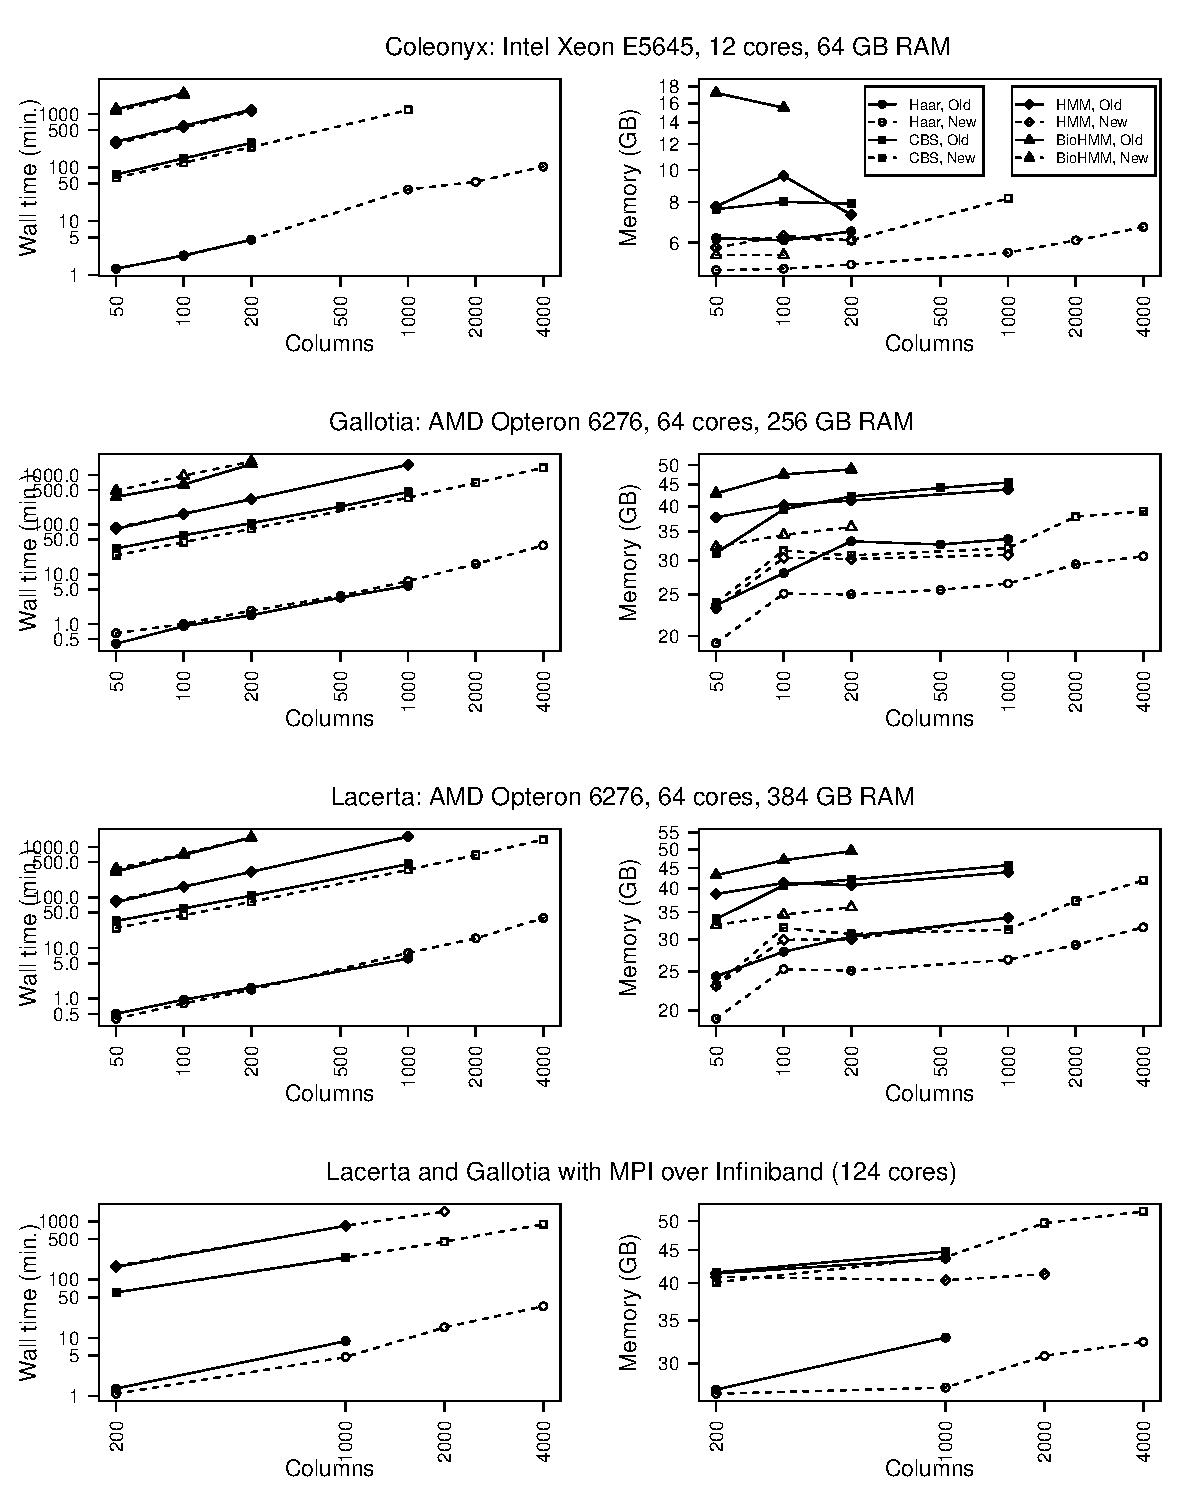
\includegraphics[width=16.1cm,keepaspectratio]{anal-benchmark-fig.pdf}
\end{center}
\caption[Wall time and memory usage when analyzing data: version
comparison]{\label{fig-anal} Comparison between old and new version in
  wall time and memory usage as a function of number of columns
  (samples). Both axis shown in log scale. The figure shows the default
  use cases: using 12 cores in the Intel Xeon machine and 64 cores in the
  AMD Opterons. Since the old version assumes no missing data, when
  possible (i.e., when data read by the old version are available) the
  data without missing values have been used with option
  \texttt{certain\_noNA = TRUE}; these correspond to rows labeled
  ``New-noNA'' in tables \ref{anal-coleonyx} to
  \ref{anal-lacerta-gallotia}. When more than one benchmark is available
  for a scenario, the median is shown.}
\end{figure}



\begin{landscape}
\begin{center}
% mylatex(tmp <- with(all.run, {     tmp2 <- all.run[all.run$machine == "Coleonyx", ]     cols <- c(1:5, 7, 6, 8:10)     tmp4 <- with(tmp2, {         tmp3 <- tmp2[order(method, ncols, Version_ADaCGH2, MPI,              numcores, universesize), cols]         rownames(tmp3) <- 1:nrow(tmp3)         tmp3     })     attributes(tmp4)$mycolnames <- attributes(all.run)$mycolnames[cols]     tmp4 }), rowlabel = "", colheads = attributes(tmp)$mycolnames, longtable = TRUE,      lines.page = 900, caption = "Analysis benchmarks for Coleonyx: Intel Xeon E5645, 12 cores, 64 GB RAM",      file = "anal-coleonyx.tex") 
%

\setlongtables


\begin{longtable}{lrrrlrlrrrl}\caption{Analysis benchmarks for Coleonyx: Intel Xeon E5645, 12 cores, 64 GB RAM} \tabularnewline
\hline\hline
\multicolumn{1}{l}{}&\multicolumn{1}{c}{Wall time (min.)}&\multicolumn{1}{c}{Memory (GB)}&\multicolumn{1}{c}{$\Sigma$ Memory (GB)}&\multicolumn{1}{c}{Method}&\multicolumn{1}{c}{Columns}&\multicolumn{1}{c}{MPI/Fork}&\multicolumn{1}{c}{Cores}&\multicolumn{1}{c}{Procs.\ per node}&\multicolumn{1}{c}{Universe size}&\multicolumn{1}{c}{Version}\tabularnewline
\hline
\endfirsthead\caption[]{\em (Analysis benchmarks for Coleonyx: Intel Xeon E5645, 12 cores, 64 GB RAM, continued)} \tabularnewline
\hline
\multicolumn{1}{l}{}&\multicolumn{1}{c}{Wall time (min.)}&\multicolumn{1}{c}{Memory (GB)}&\multicolumn{1}{c}{$\Sigma$ Memory (GB)}&\multicolumn{1}{c}{Method}&\multicolumn{1}{c}{Columns}&\multicolumn{1}{c}{MPI/Fork}&\multicolumn{1}{c}{Cores}&\multicolumn{1}{c}{Procs.\ per node}&\multicolumn{1}{c}{Universe size}&\multicolumn{1}{c}{Version}\tabularnewline
\hline
\endhead
\hline
\endfoot
\label{anal-coleonyx}
1&$   2.0$&$0.13$&$ 5.3$&Haar&$  50$&Fork&$12$&$$&$$&New\tabularnewline
2&$   1.8$&$0.13$&$ 5.2$&Haar&$  50$&Fork-LB&$12$&$$&$$&New\tabularnewline
3&$   1.4$&$0.13$&$ 5.0$&Haar&$  50$&Fork&$12$&$$&$$&New-noNA\tabularnewline
4&$   1.2$&$0.13$&$ 4.9$&Haar&$  50$&Fork&$12$&$$&$$&New-noNA\tabularnewline
5&$   1.6$&$0.13$&$ 4.9$&Haar&$  50$&Fork-LB&$12$&$$&$$&New-noNA\tabularnewline
6&$   1.4$&$0.16$&$ 5.8$&Haar&$  50$&MPI&$$&$12$&$11$&Old\tabularnewline
7&$   1.3$&$0.16$&$ 6.2$&Haar&$  50$&MPI&$$&$13$&$12$&Old\tabularnewline
8&$   1.2$&$0.16$&$ 6.4$&Haar&$  50$&MPI&$$&$13$&$12$&Old\tabularnewline
9&$   3.1$&$0.14$&$ 5.2$&Haar&$ 100$&Fork&$12$&$$&$$&New\tabularnewline
10&$   3.2$&$0.13$&$ 5.1$&Haar&$ 100$&Fork-LB&$12$&$$&$$&New\tabularnewline
11&$   2.8$&$0.13$&$ 3.2$&Haar&$ 100$&MPI&$$&$12$&$11$&New\tabularnewline
12&$   3.1$&$0.13$&$ 5.2$&Haar&$ 100$&MPI-LB&$$&$12$&$11$&New\tabularnewline
13&$   2.3$&$0.13$&$ 5.0$&Haar&$ 100$&Fork&$12$&$$&$$&New-noNA\tabularnewline
14&$   2.2$&$0.13$&$ 5.0$&Haar&$ 100$&Fork&$12$&$$&$$&New-noNA\tabularnewline
15&$   2.7$&$0.13$&$ 5.0$&Haar&$ 100$&Fork-LB&$12$&$$&$$&New-noNA\tabularnewline
16&$   2.6$&$0.17$&$ 5.9$&Haar&$ 100$&MPI&$$&$12$&$11$&Old\tabularnewline
17&$   2.3$&$0.17$&$ 6.1$&Haar&$ 100$&MPI&$$&$13$&$12$&Old\tabularnewline
18&$   2.3$&$0.17$&$ 6.1$&Haar&$ 100$&MPI&$$&$13$&$12$&Old\tabularnewline
19&$   5.8$&$0.13$&$ 5.2$&Haar&$ 200$&Fork&$12$&$$&$$&New\tabularnewline
20&$   5.3$&$0.13$&$ 5.4$&Haar&$ 200$&Fork-LB&$12$&$$&$$&New\tabularnewline
21&$   7.9$&$0.13$&$ 5.3$&Haar&$ 200$&MPI&$$&$12$&$11$&New\tabularnewline
22&$   5.7$&$0.13$&$ 5.6$&Haar&$ 200$&MPI-LB&$$&$12$&$11$&New\tabularnewline
23&$   4.8$&$0.13$&$ 5.3$&Haar&$ 200$&Fork&$12$&$$&$$&New-noNA\tabularnewline
24&$   4.2$&$0.13$&$ 5.0$&Haar&$ 200$&Fork&$12$&$$&$$&New-noNA\tabularnewline
25&$   5.3$&$0.13$&$ 5.0$&Haar&$ 200$&Fork-LB&$12$&$$&$$&New-noNA\tabularnewline
26&$   6.7$&$0.13$&$ 5.2$&Haar&$ 200$&MPI&$$&$12$&$11$&New-noNA\tabularnewline
27&$   5.2$&$0.13$&$ 5.1$&Haar&$ 200$&MPI-LB&$$&$12$&$11$&New-noNA\tabularnewline
28&$   4.8$&$0.18$&$ 6.0$&Haar&$ 200$&MPI&$$&$12$&$11$&Old\tabularnewline
29&$   4.5$&$0.18$&$ 6.5$&Haar&$ 200$&MPI&$$&$13$&$12$&Old\tabularnewline
30&$   4.3$&$0.18$&$ 6.5$&Haar&$ 200$&MPI&$$&$13$&$12$&Old\tabularnewline
31&$  38.9$&$0.14$&$ 5.6$&Haar&$1000$&Fork&$12$&$$&$$&New\tabularnewline
32&$  29.8$&$0.14$&$ 5.7$&Haar&$1000$&Fork-LB&$12$&$$&$$&New\tabularnewline
33&$  38.7$&$0.14$&$ 5.7$&Haar&$1000$&MPI&$$&$12$&$11$&New\tabularnewline
34&$  29.8$&$0.14$&$10.0$&Haar&$1000$&MPI-LB&$$&$12$&$11$&New\tabularnewline
35&$  54.2$&$0.15$&$ 6.1$&Haar&$2000$&Fork&$12$&$$&$$&New\tabularnewline
36&$  58.6$&$0.15$&$ 6.1$&Haar&$2000$&Fork-LB&$12$&$$&$$&New\tabularnewline
37&$ 104.1$&$0.18$&$ 6.7$&Haar&$4000$&Fork&$12$&$$&$$&New\tabularnewline
38&$ 117.3$&$0.18$&$ 6.3$&Haar&$4000$&Fork-LB&$12$&$$&$$&New\tabularnewline
39&$  69.7$&$0.13$&$ 7.5$&CBS&$  50$&Fork&$12$&$$&$$&New\tabularnewline
40&$  64.5$&$0.13$&$ 7.1$&CBS&$  50$&Fork-LB&$12$&$$&$$&New\tabularnewline
41&$  70.0$&$0.13$&$ 6.8$&CBS&$  50$&Fork&$12$&$$&$$&New-noNA\tabularnewline
42&$  68.3$&$0.13$&$ 6.6$&CBS&$  50$&Fork&$12$&$$&$$&New-noNA\tabularnewline
43&$  70.9$&$0.13$&$ 6.8$&CBS&$  50$&Fork&$12$&$$&$$&New-noNA\tabularnewline
44&$  64.6$&$0.13$&$ 6.2$&CBS&$  50$&Fork-LB&$12$&$$&$$&New-noNA\tabularnewline
45&$  74.2$&$0.13$&$ 7.6$&CBS&$  50$&MPI&$$&$12$&$11$&Old\tabularnewline
46&$  74.1$&$0.13$&$ 7.6$&CBS&$  50$&MPI&$$&$12$&$11$&Old\tabularnewline
47&$  77.3$&$0.13$&$ 8.1$&CBS&$  50$&MPI&$$&$13$&$12$&Old\tabularnewline
48&$ 133.5$&$0.13$&$ 9.8$&CBS&$ 100$&Fork&$12$&$$&$$&New\tabularnewline
49&$ 124.2$&$0.13$&$ 7.2$&CBS&$ 100$&Fork-LB&$12$&$$&$$&New\tabularnewline
50&$ 132.4$&$0.13$&$ 8.4$&CBS&$ 100$&Fork&$12$&$$&$$&New-noNA\tabularnewline
51&$ 131.2$&$0.13$&$ 7.2$&CBS&$ 100$&Fork&$12$&$$&$$&New-noNA\tabularnewline
52&$ 122.7$&$0.13$&$ 6.2$&CBS&$ 100$&Fork-LB&$12$&$$&$$&New-noNA\tabularnewline
53&$ 146.2$&$0.13$&$ 8.0$&CBS&$ 100$&MPI&$$&$12$&$11$&Old\tabularnewline
54&$ 147.9$&$0.13$&$ 7.7$&CBS&$ 100$&MPI&$$&$12$&$11$&Old\tabularnewline
55&$ 150.0$&$0.13$&$15.5$&CBS&$ 100$&MPI&$$&$13$&$12$&Old\tabularnewline
56&$ 250.8$&$0.13$&$ 8.2$&CBS&$ 200$&Fork&$12$&$$&$$&New\tabularnewline
57&$ 241.4$&$0.13$&$ 7.5$&CBS&$ 200$&Fork-LB&$12$&$$&$$&New\tabularnewline
58&$ 380.0$&$0.13$&$ 9.0$&CBS&$ 200$&MPI&$$&$12$&$11$&New\tabularnewline
59&$ 307.9$&$0.13$&$ 8.4$&CBS&$ 200$&MPI-LB&$$&$12$&$11$&New\tabularnewline
60&$ 255.2$&$0.13$&$14.2$&CBS&$ 200$&Fork&$12$&$$&$$&New-noNA\tabularnewline
61&$ 250.7$&$0.13$&$ 7.3$&CBS&$ 200$&Fork&$12$&$$&$$&New-noNA\tabularnewline
62&$ 240.3$&$0.13$&$ 6.1$&CBS&$ 200$&Fork-LB&$12$&$$&$$&New-noNA\tabularnewline
63&$ 372.4$&$0.13$&$ 8.7$&CBS&$ 200$&MPI&$$&$12$&$11$&New-noNA\tabularnewline
64&$ 307.8$&$0.13$&$ 7.9$&CBS&$ 200$&MPI-LB&$$&$12$&$11$&New-noNA\tabularnewline
65&$ 287.7$&$0.13$&$ 7.9$&CBS&$ 200$&MPI&$$&$12$&$11$&Old\tabularnewline
66&$ 287.2$&$0.13$&$ 7.2$&CBS&$ 200$&MPI&$$&$12$&$11$&Old\tabularnewline
67&$ 294.6$&$0.13$&$10.6$&CBS&$ 200$&MPI&$$&$13$&$12$&Old\tabularnewline
68&$1246.0$&$0.14$&$14.8$&CBS&$1000$&Fork&$12$&$$&$$&New\tabularnewline
69&$1185.2$&$0.14$&$ 8.2$&CBS&$1000$&Fork-LB&$12$&$$&$$&New\tabularnewline
70&$1804.2$&$0.14$&$10.0$&CBS&$1000$&MPI&$$&$12$&$11$&New\tabularnewline
71&$1512.4$&$0.14$&$ 8.9$&CBS&$1000$&MPI-LB&$$&$12$&$11$&New\tabularnewline
72&$ 311.2$&$0.18$&$ 6.4$&HMM&$  50$&Fork&$11$&$$&$$&New\tabularnewline
73&$ 309.5$&$0.18$&$10.5$&HMM&$  50$&Fork&$11$&$$&$$&New\tabularnewline
74&$ 282.1$&$0.18$&$ 7.0$&HMM&$  50$&Fork&$12$&$$&$$&New\tabularnewline
75&$ 286.4$&$0.18$&$ 7.1$&HMM&$  50$&Fork&$12$&$$&$$&New\tabularnewline
76&$ 288.4$&$0.18$&$ 9.6$&HMM&$  50$&Fork&$12$&$$&$$&New\tabularnewline
77&$ 281.0$&$0.18$&$ 6.3$&HMM&$  50$&Fork-LB&$12$&$$&$$&New\tabularnewline
78&$ 310.9$&$0.18$&$ 9.1$&HMM&$  50$&Fork&$12$&$$&$$&New-noNA\tabularnewline
79&$ 284.0$&$0.18$&$11.5$&HMM&$  50$&Fork&$12$&$$&$$&New-noNA\tabularnewline
80&$ 280.1$&$0.18$&$ 5.8$&HMM&$  50$&Fork-LB&$12$&$$&$$&New-noNA\tabularnewline
81&$ 322.5$&$0.18$&$ 7.2$&HMM&$  50$&MPI&$$&$11$&$10$&Old\tabularnewline
82&$ 324.4$&$0.18$&$ 7.2$&HMM&$  50$&MPI&$$&$11$&$10$&Old\tabularnewline
83&$ 298.2$&$0.18$&$ 7.3$&HMM&$  50$&MPI&$$&$12$&$11$&Old\tabularnewline
84&$ 302.2$&$0.18$&$10.2$&HMM&$  50$&MPI&$$&$12$&$11$&Old\tabularnewline
85&$ 299.9$&$0.18$&$ 8.2$&HMM&$  50$&MPI&$$&$13$&$12$&Old\tabularnewline
86&$ 305.8$&$0.18$&$ 9.8$&HMM&$  50$&MPI&$$&$13$&$12$&Old\tabularnewline
87&$ 574.2$&$0.18$&$ 9.5$&HMM&$ 100$&Fork&$12$&$$&$$&New\tabularnewline
88&$ 552.2$&$0.18$&$ 6.4$&HMM&$ 100$&Fork-LB&$12$&$$&$$&New\tabularnewline
89&$ 560.4$&$0.18$&$11.3$&HMM&$ 100$&Fork&$12$&$$&$$&New-noNA\tabularnewline
90&$ 559.1$&$0.18$&$ 6.3$&HMM&$ 100$&Fork-LB&$12$&$$&$$&New-noNA\tabularnewline
91&$ 603.0$&$0.18$&$10.7$&HMM&$ 100$&MPI&$$&$12$&$11$&Old\tabularnewline
92&$ 595.4$&$0.18$&$ 8.5$&HMM&$ 100$&MPI&$$&$13$&$12$&Old\tabularnewline
93&$1117.5$&$0.18$&$ 6.1$&HMM&$ 200$&Fork-LB&$12$&$$&$$&New\tabularnewline
94&$3188.2$&$0.20$&$ 8.7$&HMM&$ 200$&MPI&$$&$12$&$11$&New\tabularnewline
95&$1213.7$&$0.20$&$ 8.1$&HMM&$ 200$&MPI-LB&$$&$12$&$11$&New\tabularnewline
96&$1108.7$&$0.18$&$ 7.9$&HMM&$ 200$&Fork&$12$&$$&$$&New-noNA\tabularnewline
97&$1122.8$&$0.18$&$13.5$&HMM&$ 200$&Fork&$12$&$$&$$&New-noNA\tabularnewline
98&$1112.3$&$0.18$&$ 6.1$&HMM&$ 200$&Fork-LB&$12$&$$&$$&New-noNA\tabularnewline
99&$3240.6$&$0.20$&$ 9.1$&HMM&$ 200$&MPI&$$&$12$&$11$&New-noNA\tabularnewline
100&$1205.0$&$0.20$&$ 8.4$&HMM&$ 200$&MPI-LB&$$&$12$&$11$&New-noNA\tabularnewline
101&$1192.3$&$0.20$&$ 7.3$&HMM&$ 200$&MPI&$$&$12$&$11$&Old\tabularnewline
102&$1169.4$&$0.18$&$10.5$&BioHMM&$  50$&Fork&$12$&$$&$$&New-noNA\tabularnewline
103&$1122.9$&$0.18$&$ 5.5$&BioHMM&$  50$&Fork-LB&$12$&$$&$$&New-noNA\tabularnewline
104&$1222.2$&$0.18$&$17.2$&BioHMM&$  50$&MPI&$$&$13$&$12$&Old\tabularnewline
105&$2339.5$&$0.18$&$11.0$&BioHMM&$ 100$&Fork&$12$&$$&$$&New-noNA\tabularnewline
106&$2235.4$&$0.18$&$ 5.5$&BioHMM&$ 100$&Fork-LB&$12$&$$&$$&New-noNA\tabularnewline
107&$2401.8$&$0.18$&$15.5$&BioHMM&$ 100$&MPI&$$&$13$&$12$&Old\tabularnewline
\hline
\end{longtable}


\clearpage
% mylatex(tmp <- with(all.run, {     tmp2 <- all.run[all.run$machine == "Gallotia", ]     cols <- c(1:5, 7, 6, 8:10)     tmp4 <- with(tmp2, {         tmp3 <- tmp2[order(method, ncols, Version_ADaCGH2, MPI,              numcores, universesize), cols]         rownames(tmp3) <- 1:nrow(tmp3)         tmp3     })     attributes(tmp4)$mycolnames <- attributes(all.run)$mycolnames[cols]     tmp4 }), rowlabel = "", colheads = attributes(tmp)$mycolnames, longtable = TRUE,      lines.page = 900, caption = "Analysis benchmarks for Gallotia: AMD Opteron 6276, 64 cores, 256 GB RAM",      file = "anal-gallotia.tex") 
%

\setlongtables


\begin{longtable}{lrrrlrlrrrl}\caption{Analysis benchmarks for Gallotia: AMD Opteron 6276, 64 cores, 256 GB RAM} \tabularnewline
\hline\hline
\multicolumn{1}{l}{}&\multicolumn{1}{c}{Wall time (min.)}&\multicolumn{1}{c}{Memory (GB)}&\multicolumn{1}{c}{$\Sigma$ Memory (GB)}&\multicolumn{1}{c}{Method}&\multicolumn{1}{c}{Columns}&\multicolumn{1}{c}{MPI/Fork}&\multicolumn{1}{c}{Cores}&\multicolumn{1}{c}{Procs.\ per node}&\multicolumn{1}{c}{Universe size}&\multicolumn{1}{c}{Version}\tabularnewline
\hline
\endfirsthead\caption[]{\em (Analysis benchmarks for Gallotia: AMD Opteron 6276, 64 cores, 256 GB RAM, continued)} \tabularnewline
\hline
\multicolumn{1}{l}{}&\multicolumn{1}{c}{Wall time (min.)}&\multicolumn{1}{c}{Memory (GB)}&\multicolumn{1}{c}{$\Sigma$ Memory (GB)}&\multicolumn{1}{c}{Method}&\multicolumn{1}{c}{Columns}&\multicolumn{1}{c}{MPI/Fork}&\multicolumn{1}{c}{Cores}&\multicolumn{1}{c}{Procs.\ per node}&\multicolumn{1}{c}{Universe size}&\multicolumn{1}{c}{Version}\tabularnewline
\hline
\endhead
\hline
\endfoot
\label{anal-gallotia}
1&$   0.7$&$0.13$&$20.2$&Haar&$  50$&Fork&$64$&$$&$$&New\tabularnewline
2&$   1.4$&$0.13$&$18.6$&Haar&$  50$&Fork-LB&$64$&$$&$$&New\tabularnewline
3&$   0.6$&$0.13$&$19.2$&Haar&$  50$&Fork&$64$&$$&$$&New-noNA\tabularnewline
4&$   0.7$&$0.13$&$19.3$&Haar&$  50$&Fork&$64$&$$&$$&New-noNA\tabularnewline
5&$   0.6$&$0.13$&$19.2$&Haar&$  50$&Fork-LB&$64$&$$&$$&New-noNA\tabularnewline
6&$   0.4$&$0.16$&$23.6$&Haar&$  50$&MPI&$$&$64$&$63$&Old\tabularnewline
7&$   1.2$&$0.13$&$25.7$&Haar&$ 100$&Fork&$64$&$$&$$&New\tabularnewline
8&$   1.9$&$0.13$&$23.6$&Haar&$ 100$&Fork-LB&$64$&$$&$$&New\tabularnewline
9&$   1.0$&$0.13$&$25.2$&Haar&$ 100$&Fork&$64$&$$&$$&New-noNA\tabularnewline
10&$   1.0$&$0.13$&$25.0$&Haar&$ 100$&Fork&$64$&$$&$$&New-noNA\tabularnewline
11&$   1.1$&$0.13$&$24.5$&Haar&$ 100$&Fork-LB&$64$&$$&$$&New-noNA\tabularnewline
12&$   0.8$&$0.17$&$28.1$&Haar&$ 100$&MPI&$$&$64$&$63$&Old\tabularnewline
13&$   0.9$&$0.17$&$28.0$&Haar&$ 100$&MPI&$$&$65$&$64$&Old\tabularnewline
14&$   0.9$&$0.17$&$27.8$&Haar&$ 100$&MPI&$$&$65$&$64$&Old\tabularnewline
15&$   2.4$&$0.13$&$25.8$&Haar&$ 200$&Fork&$64$&$$&$$&New\tabularnewline
16&$   2.8$&$0.13$&$25.2$&Haar&$ 200$&Fork-LB&$64$&$$&$$&New\tabularnewline
17&$   2.6$&$0.14$&$28.3$&Haar&$ 200$&MPI&$$&$64$&$63$&New\tabularnewline
18&$   1.9$&$0.14$&$28.1$&Haar&$ 200$&MPI-LB&$$&$64$&$63$&New\tabularnewline
19&$   1.9$&$0.14$&$25.0$&Haar&$ 200$&Fork&$64$&$$&$$&New-noNA\tabularnewline
20&$   1.8$&$0.14$&$25.0$&Haar&$ 200$&Fork&$64$&$$&$$&New-noNA\tabularnewline
21&$   1.9$&$0.13$&$24.7$&Haar&$ 200$&Fork-LB&$64$&$$&$$&New-noNA\tabularnewline
22&$   2.7$&$0.14$&$27.1$&Haar&$ 200$&MPI&$$&$64$&$63$&New-noNA\tabularnewline
23&$   1.8$&$0.14$&$26.7$&Haar&$ 200$&MPI-LB&$$&$64$&$63$&New-noNA\tabularnewline
24&$   1.4$&$0.18$&$34.2$&Haar&$ 200$&MPI&$$&$64$&$63$&Old\tabularnewline
25&$   1.6$&$0.18$&$33.2$&Haar&$ 200$&MPI&$$&$65$&$64$&Old\tabularnewline
26&$   1.5$&$0.18$&$32.6$&Haar&$ 200$&MPI&$$&$65$&$64$&Old\tabularnewline
27&$   3.7$&$0.13$&$27.0$&Haar&$ 500$&Fork&$64$&$$&$$&New\tabularnewline
28&$   3.7$&$0.14$&$25.6$&Haar&$ 500$&Fork&$64$&$$&$$&New-noNA\tabularnewline
29&$   3.8$&$0.18$&$31.3$&Haar&$ 500$&MPI&$$&$64$&$63$&Old\tabularnewline
30&$   3.0$&$0.18$&$34.0$&Haar&$ 500$&MPI&$$&$64$&$63$&Old\tabularnewline
31&$   7.0$&$0.14$&$27.7$&Haar&$1000$&Fork&$64$&$$&$$&New\tabularnewline
32&$  10.1$&$0.14$&$27.5$&Haar&$1000$&Fork&$64$&$$&$$&New\tabularnewline
33&$  13.0$&$0.14$&$26.4$&Haar&$1000$&Fork-LB&$64$&$$&$$&New\tabularnewline
34&$  10.2$&$0.14$&$27.4$&Haar&$1000$&Fork-LB&$64$&$$&$$&New\tabularnewline
35&$  12.4$&$0.14$&$29.3$&Haar&$1000$&MPI&$$&$64$&$63$&New\tabularnewline
36&$   8.9$&$0.14$&$28.6$&Haar&$1000$&MPI-LB&$$&$64$&$63$&New\tabularnewline
37&$   6.5$&$0.14$&$26.3$&Haar&$1000$&Fork&$64$&$$&$$&New-noNA\tabularnewline
38&$   8.9$&$0.14$&$26.6$&Haar&$1000$&Fork&$64$&$$&$$&New-noNA\tabularnewline
39&$   7.3$&$0.14$&$26.5$&Haar&$1000$&Fork&$64$&$$&$$&New-noNA\tabularnewline
40&$   7.6$&$0.14$&$25.9$&Haar&$1000$&Fork-LB&$64$&$$&$$&New-noNA\tabularnewline
41&$   8.7$&$0.14$&$25.8$&Haar&$1000$&Fork-LB&$64$&$$&$$&New-noNA\tabularnewline
42&$   6.2$&$0.14$&$28.7$&Haar&$1000$&MPI&$$&$64$&$63$&New-noNA\tabularnewline
43&$   6.2$&$0.14$&$28.5$&Haar&$1000$&MPI-LB&$$&$64$&$63$&New-noNA\tabularnewline
44&$   5.9$&$0.18$&$33.6$&Haar&$1000$&MPI&$$&$64$&$63$&Old\tabularnewline
45&$  15.3$&$0.15$&$28.9$&Haar&$2000$&Fork&$64$&$$&$$&New\tabularnewline
46&$  16.9$&$0.15$&$29.8$&Haar&$2000$&Fork&$64$&$$&$$&New\tabularnewline
47&$  21.8$&$0.15$&$28.4$&Haar&$2000$&Fork-LB&$64$&$$&$$&New\tabularnewline
48&$  19.9$&$0.15$&$29.1$&Haar&$2000$&Fork-LB&$64$&$$&$$&New\tabularnewline
49&$  35.6$&$0.18$&$30.7$&Haar&$4000$&Fork&$64$&$$&$$&New\tabularnewline
50&$  40.8$&$0.18$&$30.6$&Haar&$4000$&Fork&$64$&$$&$$&New\tabularnewline
51&$  43.2$&$0.18$&$29.1$&Haar&$4000$&Fork-LB&$64$&$$&$$&New\tabularnewline
52&$  39.9$&$0.18$&$30.2$&Haar&$4000$&Fork-LB&$64$&$$&$$&New\tabularnewline
53&$  25.1$&$0.13$&$29.2$&CBS&$  50$&Fork&$64$&$$&$$&New\tabularnewline
54&$  24.3$&$0.14$&$27.9$&CBS&$  50$&Fork-LB&$64$&$$&$$&New\tabularnewline
55&$  25.1$&$0.13$&$23.8$&CBS&$  50$&Fork&$64$&$$&$$&New-noNA\tabularnewline
56&$  24.7$&$0.13$&$23.8$&CBS&$  50$&Fork&$64$&$$&$$&New-noNA\tabularnewline
57&$  24.0$&$0.13$&$23.9$&CBS&$  50$&Fork-LB&$64$&$$&$$&New-noNA\tabularnewline
58&$  33.1$&$0.13$&$31.2$&CBS&$  50$&MPI&$$&$64$&$63$&Old\tabularnewline
59&$  47.7$&$0.13$&$37.1$&CBS&$ 100$&Fork&$64$&$$&$$&New\tabularnewline
60&$  45.1$&$0.14$&$36.3$&CBS&$ 100$&Fork-LB&$64$&$$&$$&New\tabularnewline
61&$  48.2$&$0.13$&$31.1$&CBS&$ 100$&Fork&$64$&$$&$$&New-noNA\tabularnewline
62&$  47.0$&$0.14$&$30.4$&CBS&$ 100$&Fork&$64$&$$&$$&New-noNA\tabularnewline
63&$  44.6$&$0.13$&$31.6$&CBS&$ 100$&Fork-LB&$64$&$$&$$&New-noNA\tabularnewline
64&$  60.3$&$0.13$&$38.8$&CBS&$ 100$&MPI&$$&$64$&$63$&Old\tabularnewline
65&$  61.2$&$0.13$&$39.4$&CBS&$ 100$&MPI&$$&$65$&$64$&Old\tabularnewline
66&$  61.6$&$0.13$&$39.7$&CBS&$ 100$&MPI&$$&$65$&$64$&Old\tabularnewline
67&$  87.5$&$0.13$&$38.7$&CBS&$ 200$&Fork&$64$&$$&$$&New\tabularnewline
68&$  82.9$&$0.14$&$37.4$&CBS&$ 200$&Fork-LB&$64$&$$&$$&New\tabularnewline
69&$ 134.6$&$0.14$&$44.2$&CBS&$ 200$&MPI&$$&$64$&$63$&New\tabularnewline
70&$ 104.1$&$0.14$&$44.3$&CBS&$ 200$&MPI-LB&$$&$64$&$63$&New\tabularnewline
71&$  88.9$&$0.13$&$34.1$&CBS&$ 200$&Fork&$64$&$$&$$&New-noNA\tabularnewline
72&$  87.0$&$0.13$&$34.4$&CBS&$ 200$&Fork&$64$&$$&$$&New-noNA\tabularnewline
73&$  82.5$&$0.13$&$30.8$&CBS&$ 200$&Fork-LB&$64$&$$&$$&New-noNA\tabularnewline
74&$ 135.0$&$0.14$&$41.6$&CBS&$ 200$&MPI&$$&$64$&$63$&New-noNA\tabularnewline
75&$ 104.7$&$0.14$&$41.9$&CBS&$ 200$&MPI-LB&$$&$64$&$63$&New-noNA\tabularnewline
76&$ 106.6$&$0.13$&$41.7$&CBS&$ 200$&MPI&$$&$64$&$63$&Old\tabularnewline
77&$ 108.7$&$0.13$&$43.0$&CBS&$ 200$&MPI&$$&$65$&$64$&Old\tabularnewline
78&$ 107.5$&$0.13$&$42.2$&CBS&$ 200$&MPI&$$&$65$&$64$&Old\tabularnewline
79&$ 184.6$&$0.13$&$40.7$&CBS&$ 500$&Fork&$64$&$$&$$&New\tabularnewline
80&$ 182.6$&$0.14$&$36.8$&CBS&$ 500$&Fork&$64$&$$&$$&New-noNA\tabularnewline
81&$ 231.6$&$0.14$&$44.2$&CBS&$ 500$&MPI&$$&$64$&$63$&Old\tabularnewline
82&$ 362.5$&$0.14$&$42.1$&CBS&$1000$&Fork&$64$&$$&$$&New\tabularnewline
83&$ 355.1$&$0.14$&$36.3$&CBS&$1000$&Fork-LB&$64$&$$&$$&New\tabularnewline
84&$ 356.6$&$0.14$&$36.8$&CBS&$1000$&Fork-LB&$64$&$$&$$&New\tabularnewline
85&$ 563.2$&$0.14$&$50.9$&CBS&$1000$&MPI&$$&$64$&$63$&New\tabularnewline
86&$ 447.6$&$0.14$&$49.1$&CBS&$1000$&MPI-LB&$$&$64$&$63$&New\tabularnewline
87&$ 358.9$&$0.14$&$39.3$&CBS&$1000$&Fork&$64$&$$&$$&New-noNA\tabularnewline
88&$ 352.1$&$0.14$&$32.0$&CBS&$1000$&Fork-LB&$64$&$$&$$&New-noNA\tabularnewline
89&$ 446.7$&$0.14$&$45.6$&CBS&$1000$&MPI-LB&$$&$64$&$63$&New-noNA\tabularnewline
90&$ 455.5$&$0.14$&$45.5$&CBS&$1000$&MPI&$$&$64$&$63$&Old\tabularnewline
91&$ 722.7$&$0.16$&$43.8$&CBS&$2000$&Fork&$64$&$$&$$&New\tabularnewline
92&$ 696.4$&$0.16$&$37.9$&CBS&$2000$&Fork-LB&$64$&$$&$$&New\tabularnewline
93&$1499.6$&$0.18$&$44.2$&CBS&$4000$&Fork&$64$&$$&$$&New\tabularnewline
94&$1396.8$&$0.18$&$39.0$&CBS&$4000$&Fork-LB&$64$&$$&$$&New\tabularnewline
95&$  87.6$&$0.18$&$25.8$&HMM&$  50$&Fork-LB&$64$&$$&$$&New\tabularnewline
96&$ 105.9$&$0.17$&$30.0$&HMM&$  50$&Fork&$64$&$$&$$&New-noNA\tabularnewline
97&$  94.5$&$0.17$&$30.0$&HMM&$  50$&Fork&$64$&$$&$$&New-noNA\tabularnewline
98&$  87.2$&$0.18$&$23.2$&HMM&$  50$&Fork-LB&$64$&$$&$$&New-noNA\tabularnewline
99&$  83.0$&$0.18$&$37.9$&HMM&$  50$&MPI&$$&$64$&$63$&Old\tabularnewline
100&$  82.2$&$0.18$&$37.6$&HMM&$  50$&MPI&$$&$64$&$63$&Old\tabularnewline
101&$ 175.7$&$0.18$&$33.6$&HMM&$ 100$&Fork&$63$&$$&$$&New\tabularnewline
102&$ 174.2$&$0.18$&$33.4$&HMM&$ 100$&Fork&$63$&$$&$$&New\tabularnewline
103&$ 165.4$&$0.18$&$34.5$&HMM&$ 100$&Fork&$64$&$$&$$&New\tabularnewline
104&$ 166.3$&$0.18$&$34.4$&HMM&$ 100$&Fork&$64$&$$&$$&New\tabularnewline
105&$ 179.2$&$0.18$&$32.8$&HMM&$ 100$&Fork-LB&$64$&$$&$$&New\tabularnewline
106&$ 166.9$&$0.18$&$31.4$&HMM&$ 100$&Fork&$64$&$$&$$&New-noNA\tabularnewline
107&$ 168.0$&$0.18$&$31.6$&HMM&$ 100$&Fork&$64$&$$&$$&New-noNA\tabularnewline
108&$ 166.2$&$0.18$&$30.4$&HMM&$ 100$&Fork-LB&$64$&$$&$$&New-noNA\tabularnewline
109&$ 164.0$&$0.18$&$38.9$&HMM&$ 100$&MPI&$$&$63$&$62$&Old\tabularnewline
110&$ 164.6$&$0.18$&$39.6$&HMM&$ 100$&MPI&$$&$63$&$62$&Old\tabularnewline
111&$ 160.9$&$0.18$&$40.7$&HMM&$ 100$&MPI&$$&$64$&$63$&Old\tabularnewline
112&$ 163.0$&$0.18$&$39.9$&HMM&$ 100$&MPI&$$&$64$&$63$&Old\tabularnewline
113&$ 168.8$&$0.18$&$41.1$&HMM&$ 100$&MPI&$$&$65$&$64$&Old\tabularnewline
114&$ 167.9$&$0.18$&$41.4$&HMM&$ 100$&MPI&$$&$65$&$64$&Old\tabularnewline
115&$ 333.8$&$0.18$&$34.4$&HMM&$ 200$&Fork&$63$&$$&$$&New\tabularnewline
116&$ 336.5$&$0.18$&$34.8$&HMM&$ 200$&Fork&$63$&$$&$$&New\tabularnewline
117&$ 331.5$&$0.18$&$36.1$&HMM&$ 200$&Fork&$64$&$$&$$&New\tabularnewline
118&$ 333.3$&$0.18$&$36.1$&HMM&$ 200$&Fork&$64$&$$&$$&New\tabularnewline
119&$ 359.6$&$0.19$&$33.1$&HMM&$ 200$&Fork-LB&$64$&$$&$$&New\tabularnewline
120&$1110.5$&$0.20$&$40.5$&HMM&$ 200$&MPI&$$&$64$&$63$&New\tabularnewline
121&$ 329.7$&$0.20$&$41.5$&HMM&$ 200$&MPI-LB&$$&$64$&$63$&New\tabularnewline
122&$ 328.7$&$0.18$&$33.5$&HMM&$ 200$&Fork&$64$&$$&$$&New-noNA\tabularnewline
123&$ 328.9$&$0.18$&$33.6$&HMM&$ 200$&Fork&$64$&$$&$$&New-noNA\tabularnewline
124&$ 325.1$&$0.18$&$30.2$&HMM&$ 200$&Fork-LB&$64$&$$&$$&New-noNA\tabularnewline
125&$1109.4$&$0.20$&$43.1$&HMM&$ 200$&MPI&$$&$64$&$63$&New-noNA\tabularnewline
126&$ 326.9$&$0.20$&$42.8$&HMM&$ 200$&MPI-LB&$$&$64$&$63$&New-noNA\tabularnewline
127&$ 331.3$&$0.20$&$40.8$&HMM&$ 200$&MPI&$$&$63$&$62$&Old\tabularnewline
128&$ 330.2$&$0.20$&$41.1$&HMM&$ 200$&MPI&$$&$63$&$62$&Old\tabularnewline
129&$ 319.5$&$0.20$&$41.7$&HMM&$ 200$&MPI&$$&$64$&$63$&Old\tabularnewline
130&$ 325.8$&$0.20$&$41.5$&HMM&$ 200$&MPI&$$&$64$&$63$&Old\tabularnewline
131&$1616.9$&$0.21$&$40.7$&HMM&$1000$&Fork&$64$&$$&$$&New-noNA\tabularnewline
132&$1618.0$&$0.22$&$30.9$&HMM&$1000$&Fork-LB&$64$&$$&$$&New-noNA\tabularnewline
133&$1612.1$&$0.26$&$43.8$&HMM&$1000$&MPI&$$&$64$&$63$&Old\tabularnewline
134&$ 469.8$&$0.18$&$32.2$&BioHMM&$  50$&Fork&$64$&$$&$$&New-noNA\tabularnewline
135&$ 499.2$&$0.18$&$32.3$&BioHMM&$  50$&Fork&$64$&$$&$$&New-noNA\tabularnewline
136&$ 363.3$&$0.18$&$42.9$&BioHMM&$  50$&MPI&$$&$64$&$63$&Old\tabularnewline
137&$ 964.7$&$0.18$&$34.5$&BioHMM&$ 100$&Fork&$64$&$$&$$&New-noNA\tabularnewline
138&$ 979.8$&$0.18$&$34.2$&BioHMM&$ 100$&Fork&$64$&$$&$$&New-noNA\tabularnewline
139&$ 645.5$&$0.18$&$47.5$&BioHMM&$ 100$&MPI&$$&$64$&$63$&Old\tabularnewline
140&$1813.8$&$0.18$&$36.1$&BioHMM&$ 200$&Fork&$64$&$$&$$&New-noNA\tabularnewline
141&$1939.3$&$0.18$&$35.6$&BioHMM&$ 200$&Fork&$64$&$$&$$&New-noNA\tabularnewline
142&$1652.7$&$0.20$&$48.8$&BioHMM&$ 200$&MPI&$$&$64$&$63$&Old\tabularnewline
\hline
\end{longtable}


\clearpage
% mylatex(tmp <- with(all.run, {     tmp2 <- all.run[(all.run$machine == "Lacerta") & ((is.na(all.run$universesize)) |          (all.run$universesize != 124)), ]     cols <- c(1:5, 7, 6, 8:10)     tmp4 <- with(tmp2, {         tmp3 <- tmp2[order(method, ncols, Version_ADaCGH2, MPI,              numcores, universesize), cols]         rownames(tmp3) <- 1:nrow(tmp3)         tmp3     })     attributes(tmp4)$mycolnames <- attributes(all.run)$mycolnames[cols]     tmp4 }), rowlabel = "", colheads = attributes(tmp)$mycolnames, longtable = TRUE,      lines.page = 900, caption = "Analysis benchmarks for Lacerta: AMD Opteron 6276, 64 cores, 384 GB RAM",      file = "anal-lacerta.tex") 
%

\setlongtables


\begin{longtable}{lrrrlrlrrrl}\caption{Analysis benchmarks for Lacerta: AMD Opteron 6276, 64 cores, 384 GB RAM} \tabularnewline
\hline\hline
\multicolumn{1}{l}{}&\multicolumn{1}{c}{Wall time (min.)}&\multicolumn{1}{c}{Memory (GB)}&\multicolumn{1}{c}{$\Sigma$ Memory (GB)}&\multicolumn{1}{c}{Method}&\multicolumn{1}{c}{Columns}&\multicolumn{1}{c}{MPI/Fork}&\multicolumn{1}{c}{Cores}&\multicolumn{1}{c}{Procs.\ per node}&\multicolumn{1}{c}{Universe size}&\multicolumn{1}{c}{Version}\tabularnewline
\hline
\endfirsthead\caption[]{\em (Analysis benchmarks for Lacerta: AMD Opteron 6276, 64 cores, 384 GB RAM, continued)} \tabularnewline
\hline
\multicolumn{1}{l}{}&\multicolumn{1}{c}{Wall time (min.)}&\multicolumn{1}{c}{Memory (GB)}&\multicolumn{1}{c}{$\Sigma$ Memory (GB)}&\multicolumn{1}{c}{Method}&\multicolumn{1}{c}{Columns}&\multicolumn{1}{c}{MPI/Fork}&\multicolumn{1}{c}{Cores}&\multicolumn{1}{c}{Procs.\ per node}&\multicolumn{1}{c}{Universe size}&\multicolumn{1}{c}{Version}\tabularnewline
\hline
\endhead
\hline
\endfoot
\label{anal-lacerta}
1&$   0.6$&$0.13$&$20.2$&Haar&$  50$&Fork-LB&$64$&$$&$$&New\tabularnewline
2&$   0.4$&$0.13$&$19.1$&Haar&$  50$&Fork&$64$&$$&$$&New-noNA\tabularnewline
3&$   0.6$&$0.13$&$19.2$&Haar&$  50$&Fork-LB&$64$&$$&$$&New-noNA\tabularnewline
4&$   0.5$&$0.16$&$24.3$&Haar&$  50$&MPI&$$&$65$&$64$&Old\tabularnewline
5&$   0.5$&$0.16$&$24.3$&Haar&$  50$&MPI&$$&$65$&$64$&Old\tabularnewline
6&$   1.2$&$0.13$&$25.7$&Haar&$ 100$&Fork-LB&$64$&$$&$$&New\tabularnewline
7&$   0.8$&$0.13$&$25.3$&Haar&$ 100$&Fork&$64$&$$&$$&New-noNA\tabularnewline
8&$   1.1$&$0.13$&$24.5$&Haar&$ 100$&Fork-LB&$64$&$$&$$&New-noNA\tabularnewline
9&$   0.8$&$0.17$&$27.8$&Haar&$ 100$&MPI&$$&$64$&$63$&Old\tabularnewline
10&$   1.1$&$0.17$&$28.1$&Haar&$ 100$&MPI&$$&$65$&$64$&Old\tabularnewline
11&$   1.8$&$0.13$&$26.9$&Haar&$ 200$&Fork-LB&$64$&$$&$$&New\tabularnewline
12&$   2.6$&$0.13$&$28.2$&Haar&$ 200$&MPI&$$&$64$&$63$&New\tabularnewline
13&$   2.1$&$0.13$&$28.1$&Haar&$ 200$&MPI-LB&$$&$64$&$63$&New\tabularnewline
14&$   1.5$&$0.14$&$25.1$&Haar&$ 200$&Fork&$64$&$$&$$&New-noNA\tabularnewline
15&$   2.0$&$0.13$&$24.6$&Haar&$ 200$&Fork-LB&$64$&$$&$$&New-noNA\tabularnewline
16&$   2.4$&$0.13$&$27.1$&Haar&$ 200$&MPI&$$&$64$&$63$&New-noNA\tabularnewline
17&$   1.5$&$0.13$&$27.1$&Haar&$ 200$&MPI-LB&$$&$64$&$63$&New-noNA\tabularnewline
18&$   1.4$&$0.18$&$31.9$&Haar&$ 200$&MPI&$$&$64$&$63$&Old\tabularnewline
19&$   1.9$&$0.18$&$29.0$&Haar&$ 200$&MPI&$$&$65$&$64$&Old\tabularnewline
20&$  11.4$&$0.14$&$26.7$&Haar&$1000$&Fork-LB&$64$&$$&$$&New\tabularnewline
21&$  10.5$&$0.14$&$28.2$&Haar&$1000$&Fork-LB&$64$&$$&$$&New\tabularnewline
22&$  11.6$&$0.14$&$29.8$&Haar&$1000$&MPI&$$&$64$&$63$&New\tabularnewline
23&$  10.0$&$0.14$&$29.2$&Haar&$1000$&MPI-LB&$$&$64$&$63$&New\tabularnewline
24&$   8.0$&$0.14$&$26.3$&Haar&$1000$&Fork&$64$&$$&$$&New-noNA\tabularnewline
25&$   9.2$&$0.14$&$26.5$&Haar&$1000$&Fork-LB&$64$&$$&$$&New-noNA\tabularnewline
26&$   6.2$&$0.18$&$32.9$&Haar&$1000$&MPI&$$&$65$&$64$&Old\tabularnewline
27&$   6.2$&$0.18$&$34.9$&Haar&$1000$&MPI&$$&$65$&$64$&Old\tabularnewline
28&$  14.8$&$0.14$&$29.0$&Haar&$2000$&Fork&$64$&$$&$$&New\tabularnewline
29&$  21.7$&$0.14$&$27.1$&Haar&$2000$&Fork-LB&$64$&$$&$$&New\tabularnewline
30&$  36.1$&$0.18$&$32.3$&Haar&$4000$&Fork&$64$&$$&$$&New\tabularnewline
31&$  45.0$&$0.18$&$31.8$&Haar&$4000$&Fork-LB&$64$&$$&$$&New\tabularnewline
32&$  25.5$&$0.13$&$26.2$&CBS&$  50$&Fork-LB&$64$&$$&$$&New\tabularnewline
33&$  24.6$&$0.13$&$24.4$&CBS&$  50$&Fork&$64$&$$&$$&New-noNA\tabularnewline
34&$  25.0$&$0.14$&$23.1$&CBS&$  50$&Fork-LB&$64$&$$&$$&New-noNA\tabularnewline
35&$  34.0$&$0.13$&$35.0$&CBS&$  50$&MPI&$$&$65$&$64$&Old\tabularnewline
36&$  34.9$&$0.13$&$32.3$&CBS&$  50$&MPI&$$&$65$&$64$&Old\tabularnewline
37&$  44.7$&$0.13$&$34.0$&CBS&$ 100$&Fork-LB&$64$&$$&$$&New\tabularnewline
38&$  46.2$&$0.13$&$31.1$&CBS&$ 100$&Fork&$64$&$$&$$&New-noNA\tabularnewline
39&$  44.5$&$0.14$&$32.0$&CBS&$ 100$&Fork-LB&$64$&$$&$$&New-noNA\tabularnewline
40&$  61.0$&$0.13$&$40.5$&CBS&$ 100$&MPI&$$&$64$&$63$&Old\tabularnewline
41&$  60.6$&$0.13$&$41.0$&CBS&$ 100$&MPI&$$&$65$&$64$&Old\tabularnewline
42&$  83.6$&$0.13$&$35.7$&CBS&$ 200$&Fork-LB&$64$&$$&$$&New\tabularnewline
43&$ 131.5$&$0.13$&$46.1$&CBS&$ 200$&MPI&$$&$64$&$63$&New\tabularnewline
44&$ 103.3$&$0.13$&$43.9$&CBS&$ 200$&MPI-LB&$$&$64$&$63$&New\tabularnewline
45&$  88.1$&$0.14$&$34.1$&CBS&$ 200$&Fork&$64$&$$&$$&New-noNA\tabularnewline
46&$  82.1$&$0.14$&$30.9$&CBS&$ 200$&Fork-LB&$64$&$$&$$&New-noNA\tabularnewline
47&$ 134.9$&$0.13$&$43.1$&CBS&$ 200$&MPI&$$&$64$&$63$&New-noNA\tabularnewline
48&$ 102.8$&$0.13$&$42.0$&CBS&$ 200$&MPI-LB&$$&$64$&$63$&New-noNA\tabularnewline
49&$ 107.8$&$0.13$&$42.5$&CBS&$ 200$&MPI&$$&$64$&$63$&Old\tabularnewline
50&$ 109.7$&$0.13$&$41.7$&CBS&$ 200$&MPI&$$&$65$&$64$&Old\tabularnewline
51&$ 353.7$&$0.14$&$36.7$&CBS&$1000$&Fork-LB&$64$&$$&$$&New\tabularnewline
52&$ 353.4$&$0.14$&$36.4$&CBS&$1000$&Fork-LB&$64$&$$&$$&New\tabularnewline
53&$ 556.8$&$0.14$&$51.0$&CBS&$1000$&MPI&$$&$64$&$63$&New\tabularnewline
54&$ 451.2$&$0.14$&$47.9$&CBS&$1000$&MPI-LB&$$&$64$&$63$&New\tabularnewline
55&$ 359.9$&$0.14$&$38.8$&CBS&$1000$&Fork&$64$&$$&$$&New-noNA\tabularnewline
56&$ 352.3$&$0.14$&$31.7$&CBS&$1000$&Fork-LB&$64$&$$&$$&New-noNA\tabularnewline
57&$ 459.6$&$0.14$&$45.7$&CBS&$1000$&MPI&$$&$65$&$64$&Old\tabularnewline
58&$ 722.2$&$0.15$&$44.1$&CBS&$2000$&Fork&$64$&$$&$$&New\tabularnewline
59&$ 695.2$&$0.16$&$37.3$&CBS&$2000$&Fork-LB&$64$&$$&$$&New\tabularnewline
60&$1430.5$&$0.18$&$46.4$&CBS&$4000$&Fork&$64$&$$&$$&New\tabularnewline
61&$1399.4$&$0.18$&$41.9$&CBS&$4000$&Fork-LB&$64$&$$&$$&New\tabularnewline
62&$  94.5$&$0.18$&$25.8$&HMM&$  50$&Fork&$64$&$$&$$&New\tabularnewline
63&$  88.0$&$0.18$&$25.7$&HMM&$  50$&Fork-LB&$64$&$$&$$&New\tabularnewline
64&$  94.0$&$0.17$&$29.9$&HMM&$  50$&Fork&$64$&$$&$$&New-noNA\tabularnewline
65&$  86.8$&$0.18$&$23.0$&HMM&$  50$&Fork-LB&$64$&$$&$$&New-noNA\tabularnewline
66&$  81.3$&$0.18$&$38.8$&HMM&$  50$&MPI&$$&$64$&$63$&Old\tabularnewline
67&$ 166.1$&$0.18$&$32.5$&HMM&$ 100$&Fork-LB&$64$&$$&$$&New\tabularnewline
68&$ 167.1$&$0.18$&$31.7$&HMM&$ 100$&Fork&$64$&$$&$$&New-noNA\tabularnewline
69&$ 160.3$&$0.18$&$41.6$&HMM&$ 100$&MPI&$$&$64$&$63$&Old\tabularnewline
70&$ 166.5$&$0.18$&$41.0$&HMM&$ 100$&MPI&$$&$65$&$64$&Old\tabularnewline
71&$ 324.9$&$0.18$&$32.9$&HMM&$ 200$&Fork-LB&$64$&$$&$$&New\tabularnewline
72&$1113.2$&$0.20$&$41.6$&HMM&$ 200$&MPI&$$&$64$&$63$&New\tabularnewline
73&$ 326.7$&$0.20$&$40.3$&HMM&$ 200$&MPI-LB&$$&$64$&$63$&New\tabularnewline
74&$ 323.8$&$0.18$&$33.0$&HMM&$ 200$&Fork&$64$&$$&$$&New-noNA\tabularnewline
75&$1123.3$&$0.20$&$42.7$&HMM&$ 200$&MPI&$$&$64$&$63$&New-noNA\tabularnewline
76&$ 324.5$&$0.20$&$42.7$&HMM&$ 200$&MPI-LB&$$&$64$&$63$&New-noNA\tabularnewline
77&$ 322.3$&$0.20$&$40.8$&HMM&$ 200$&MPI&$$&$64$&$63$&Old\tabularnewline
78&$1612.9$&$0.21$&$40.0$&HMM&$1000$&Fork&$64$&$$&$$&New-noNA\tabularnewline
79&$1613.6$&$0.27$&$43.9$&HMM&$1000$&MPI&$$&$64$&$63$&Old\tabularnewline
80&$ 458.4$&$0.18$&$28.3$&BioHMM&$  50$&Fork&$64$&$$&$$&New\tabularnewline
81&$ 373.7$&$0.17$&$32.5$&BioHMM&$  50$&Fork&$64$&$$&$$&New-noNA\tabularnewline
82&$ 328.9$&$0.18$&$43.2$&BioHMM&$  50$&MPI&$$&$64$&$63$&Old\tabularnewline
83&$ 731.2$&$0.18$&$34.5$&BioHMM&$ 100$&Fork&$64$&$$&$$&New-noNA\tabularnewline
84&$ 697.5$&$0.18$&$47.0$&BioHMM&$ 100$&MPI&$$&$64$&$63$&Old\tabularnewline
85&$1543.5$&$0.18$&$36.0$&BioHMM&$ 200$&Fork&$64$&$$&$$&New-noNA\tabularnewline
86&$1525.2$&$0.20$&$49.5$&BioHMM&$ 200$&MPI&$$&$64$&$63$&Old\tabularnewline
\hline
\end{longtable}


\clearpage
% mylatex(tmp <- with(all.run, {     tmp2 <- all.run[(all.run$machine == "Lacerta") & ((!is.na(all.run$universesize)) &          (all.run$universesize == 124)), ]     cols <- c(1:5, 7, 6, 8:10)     tmp4 <- with(tmp2, {         tmp3 <- tmp2[order(method, ncols, Version_ADaCGH2, MPI,              numcores, universesize), cols]         rownames(tmp3) <- 1:nrow(tmp3)         tmp3     })     attributes(tmp4)$mycolnames <- attributes(all.run)$mycolnames[cols]     tmp4 }), rowlabel = "", colheads = attributes(tmp)$mycolnames, longtable = TRUE,      lines.page = 900, caption = "Analysis benchmarks using Lacerta and Gallotia with MPI over Infiniband (total 124 cores)",      file = "anal-lacerta-gallotia.tex") 
%

\setlongtables


\begin{longtable}{lrrrlrlrrrl}\caption{Analysis benchmarks using Lacerta and Gallotia with MPI over Infiniband (total 124 cores)} \tabularnewline
\hline\hline
\multicolumn{1}{l}{}&\multicolumn{1}{c}{Wall time (min.)}&\multicolumn{1}{c}{Memory (GB)}&\multicolumn{1}{c}{$\Sigma$ Memory (GB)}&\multicolumn{1}{c}{Method}&\multicolumn{1}{c}{Columns}&\multicolumn{1}{c}{MPI/Fork}&\multicolumn{1}{c}{Cores}&\multicolumn{1}{c}{Procs.\ per node}&\multicolumn{1}{c}{Universe size}&\multicolumn{1}{c}{Version}\tabularnewline
\hline
\endfirsthead\caption[]{\em (Analysis benchmarks using Lacerta and Gallotia with MPI over Infiniband (total 124 cores), continued)} \tabularnewline
\hline
\multicolumn{1}{l}{}&\multicolumn{1}{c}{Wall time (min.)}&\multicolumn{1}{c}{Memory (GB)}&\multicolumn{1}{c}{$\Sigma$ Memory (GB)}&\multicolumn{1}{c}{Method}&\multicolumn{1}{c}{Columns}&\multicolumn{1}{c}{MPI/Fork}&\multicolumn{1}{c}{Cores}&\multicolumn{1}{c}{Procs.\ per node}&\multicolumn{1}{c}{Universe size}&\multicolumn{1}{c}{Version}\tabularnewline
\hline
\endhead
\hline
\endfoot
\label{anal-lacerta-gallotia}
1&$   1.4$&$0.13$&$27.3$&Haar&$ 200$&MPI&$$&$63$&$124$&New-noNA\tabularnewline
2&$   1.3$&$0.13$&$26.9$&Haar&$ 200$&MPI&$$&$62$&$124$&New-noNA\tabularnewline
3&$   1.3$&$0.13$&$27.1$&Haar&$ 200$&MPI&$$&$62$&$124$&New-noNA\tabularnewline
4&$   1.3$&$0.13$&$27.3$&Haar&$ 200$&MPI&$$&$63$&$124$&New-noNA\tabularnewline
5&$   1.1$&$0.13$&$27.2$&Haar&$ 200$&MPI-LB&$$&$63$&$124$&New-noNA\tabularnewline
6&$   1.1$&$0.13$&$26.7$&Haar&$ 200$&MPI-LB&$$&$62$&$124$&New-noNA\tabularnewline
7&$   1.0$&$0.13$&$26.7$&Haar&$ 200$&MPI-LB&$$&$62$&$124$&New-noNA\tabularnewline
8&$   1.2$&$0.13$&$27.1$&Haar&$ 200$&MPI-LB&$$&$63$&$124$&New-noNA\tabularnewline
9&$   1.4$&$0.18$&$27.4$&Haar&$ 200$&MPI&$$&$63$&$124$&Old\tabularnewline
10&$   1.3$&$0.18$&$27.2$&Haar&$ 200$&MPI&$$&$62$&$124$&Old\tabularnewline
11&$   7.9$&$0.14$&$28.5$&Haar&$1000$&MPI&$$&$62$&$124$&New-noNA\tabularnewline
12&$   4.7$&$0.14$&$27.5$&Haar&$1000$&MPI-LB&$$&$62$&$124$&New-noNA\tabularnewline
13&$   8.8$&$0.18$&$32.9$&Haar&$1000$&MPI&$$&$62$&$124$&Old\tabularnewline
14&$  27.7$&$0.15$&$31.6$&Haar&$2000$&MPI&$$&$62$&$124$&New\tabularnewline
15&$  15.2$&$0.15$&$30.8$&Haar&$2000$&MPI-LB&$$&$62$&$124$&New\tabularnewline
16&$  59.0$&$0.18$&$31.8$&Haar&$4000$&MPI&$$&$62$&$124$&New\tabularnewline
17&$  35.0$&$0.18$&$32.4$&Haar&$4000$&MPI-LB&$$&$62$&$124$&New\tabularnewline
18&$  70.1$&$0.13$&$42.1$&CBS&$ 200$&MPI&$$&$63$&$124$&New-noNA\tabularnewline
19&$  69.6$&$0.13$&$41.4$&CBS&$ 200$&MPI&$$&$62$&$124$&New-noNA\tabularnewline
20&$  60.6$&$0.13$&$40.1$&CBS&$ 200$&MPI-LB&$$&$62$&$124$&New-noNA\tabularnewline
21&$  60.0$&$0.13$&$42.0$&CBS&$ 200$&MPI&$$&$63$&$124$&Old\tabularnewline
22&$  61.2$&$0.13$&$41.1$&CBS&$ 200$&MPI&$$&$62$&$124$&Old\tabularnewline
23&$ 324.1$&$0.14$&$44.7$&CBS&$1000$&MPI&$$&$62$&$124$&New-noNA\tabularnewline
24&$ 239.1$&$0.14$&$43.9$&CBS&$1000$&MPI-LB&$$&$62$&$124$&New-noNA\tabularnewline
25&$ 242.5$&$0.14$&$44.8$&CBS&$1000$&MPI&$$&$62$&$124$&Old\tabularnewline
26&$ 612.7$&$0.15$&$51.5$&CBS&$2000$&MPI&$$&$62$&$124$&New\tabularnewline
27&$ 452.6$&$0.15$&$49.6$&CBS&$2000$&MPI-LB&$$&$62$&$124$&New\tabularnewline
28&$1237.0$&$0.18$&$53.8$&CBS&$4000$&MPI&$$&$62$&$124$&New\tabularnewline
29&$ 893.3$&$0.18$&$51.7$&CBS&$4000$&MPI-LB&$$&$62$&$124$&New\tabularnewline
30&$ 584.2$&$0.20$&$41.8$&HMM&$ 200$&MPI&$$&$62$&$124$&New-noNA\tabularnewline
31&$ 172.1$&$0.20$&$40.9$&HMM&$ 200$&MPI-LB&$$&$62$&$124$&New-noNA\tabularnewline
32&$ 165.7$&$0.20$&$41.8$&HMM&$ 200$&MPI&$$&$63$&$124$&Old\tabularnewline
33&$ 166.4$&$0.20$&$41.0$&HMM&$ 200$&MPI&$$&$62$&$124$&Old\tabularnewline
34&$ 847.6$&$0.27$&$40.4$&HMM&$1000$&MPI-LB&$$&$62$&$124$&New-noNA\tabularnewline
35&$ 846.4$&$0.27$&$43.7$&HMM&$1000$&MPI&$$&$62$&$124$&Old\tabularnewline
36&$1489.2$&$0.35$&$41.3$&HMM&$2000$&MPI-LB&$$&$62$&$124$&New\tabularnewline
\hline
\end{longtable}


\end{center}
\end{landscape}



\section{Other comparisons}

\subsection{Comparison with non-parallelized executions}

ADaCGH2 was run without merging, to compare it to the canonical,
non-parallelized, implementations of CBS and Haar. Note that, as there are
missing values in the data, and the original HaarSeg code does not deal
with missing values, we are forced to remove NAs array-per-array, and make
repeated calls to the function.


\begin{center}
\begin{threeparttable}
  \caption[Time and memory usage of segmentation: comparison with
  non-parallized executions.]{Time and memory usage of segmentation
    without merging and comparison with non-parallized executions. These
    examples have all been run on the Dell Power Edges.}
\label{nonparall}
  \begin{tabular}{lp{1.3cm}p{1.2cm}p{1.0cm}p{0.85cm}p{1.2cm}p{1.9cm}p{1.55cm}p{1.8cm}}

    \hline\hline

&Method& MPI /Fork & Cores & ff/ RAM & Columns & Wall time (min.) & Memory
(GB)& $\Sigma$ Memory (GB)\\

\hline
\rownumber&Haar & Fork &64  & ff & 100 & 1.2   &   0.13  &  24.5  \\
\rownumber&Haar & Fork &10  & ff & 1000 &23.5 & 0.142 & 5.9 \\
\rownumber&Haar & Fork &20 & ff & 1000 & 12.3 & 0.137 & 10.0 \\
\rownumber&Haar & Fork &40  & ff & 1000 & 7.4 & 0.142 & 17.6 \\
\rownumber&Haar & Fork &50  & ff & 1000 & 6.7 & 0.139 & 21.2 \\
\rownumber&Haar & Fork & 64  & ff & 1000 & 6.4 & 0.142 & 26.9 \\

&&&&&&&\\

\rownumber&Haar & Fork &10  & ff & 2000 &49.7 & 0.16 & 8.0 \\
\rownumber&Haar & Fork &20  & ff & 2000 & 26.3 & 0.16 & 11.9 \\
\rownumber&Haar & Fork &40  & ff & 2000 & 15.4& 0.16 & 19.5 \\
\rownumber&Haar & Fork &50  & ff & 2000 & 13.3& 0.16 & 23.2 \\
\rownumber&Haar & Fork &64  & ff & 2000 & 11.9& 0.16 & 28.4 \\


&&&&&&&\\
\rownumber&CBS    & Fork & 64 & ff  & 100  & 55.9  &   0.13   &  35.3  \\
\rownumber&CBS & Fork &10  & ff & 1000 &1855.4 & 0.135 & 8.6 \\
\rownumber&CBS & Fork &20 & ff & 1000 & 939.8 & 0.135 & 14.9 \\
\rownumber&CBS & Fork &40  & ff & 1000 & 513.5 & 0.136 & 27.0 \\
\rownumber&CBS & Fork &50  & ff & 1000 & 438.6 & 0.142 & 33.1 \\
\rownumber&CBS & Fork & 64  & ff & 1000 & 350.3 & 0.142 & 41.3 \\

&&&&&&&\\
\rownumber&CBS & Fork &10  & ff & 2000 &3770.9 & 0.15 & 11.1 \\
\rownumber&CBS & Fork &20 & ff & 2000 & 1878.8 & 0.16 & 16.5 \\
\rownumber&CBS & Fork &40  & ff & 2000 & 1007.0 & 0.15 & 28.8 \\
\rownumber&CBS & Fork &50  & ff & 2000 & 857.1 & 0.16 & 35.3 \\
\rownumber&CBS & Fork & 64  & ff & 2000 & 717.3 & 0.163 & 41.9 \\

&&&&&&&\\


\rownumber&Haar & NP &-  &RAM  & 100 &  25.2\tnote{a}   & 12.5 & 12.5  \\
\rownumber&CBS     & NP &-  &RAM  & 100 & 1706\tnote{b}  &   40   &  40\\
\rownumber&Haar & NP &-  &RAM  & 1000 &
\multicolumn{3}{c}{198.3\tnote{c}\quad \textit{\textbf{Cannot allocate memory}}} \\
\rownumber&CBS     & NP &-  &RAM  & 1000 & \multicolumn{3}{c}{\textit{\qquad\textbf{Cannot allocate memory}}}\\

\hline
   
  \end{tabular}

  \begin{tablenotes}
    {\footnotesize

     \item[a] 25.25 = 0.95 + 22.9 + 1.4: load data, analyze, and save results.%  Since
      % there are missing values in the data, and the original HaarSeg code
      % does not deal with missing values, we are forced to remove NAs
      % array-per-array, and make repeated calls to the function.
      % , both o
      %  which introduce an important penalty. We must do this to make
      % analysis comparable to those of \texttt{pSegmentHaarSeg} that
      % \textbf{always} checks, and allows, for missing values. 
      If there are no missing values in this data set, the total time of
      analysis (i.e., sending the whole matrix at once and not checking
      for, nor removing, NAs) is 3.3 minutes.
    \item[b] 1706 =  0.95 + 1698 + 6.7: load data, analyze, and save results. The
      analysis involves calling the \texttt{CNA} function to create the CNA object
      (5.3 min), calling the \texttt{smooth.CNA} function to smooth the data
      and detect outlier (83.2 minutes), and segmenting the data with the
      \texttt{segment} function (1609.5 minutes).
    \item[c] The analysis uses 113 GB, but results cannot be saved.
    % \item[f] These examples have been run on the Dell Power Edges, but
    %   changing the number of cores used.
      }
  \end{tablenotes}

\end{threeparttable}
\end{center}



\subsection{Reading from a directory of files vs.\ other options}

Here we show time and memory usage of options that are not the recommended
approach with large data set (using \textit{ff} objects and reading from a
directory of single-column files). All these benchmarks have been carried
out in the AMD Opteron machines. These data show the patterns discussed in
the main vignette: with large data sets the best approach is to read from
a directory of single-column files and store as \textit{ff} objects. Wall
time is much smaller when reading from a directory of single column files
(see also table \ref{read-coleonyx} for a comparison with former versions
of ADaCGH2, where original data where stored as RData and then read to
\textit{ff} objects). Moreover, storing as a RAM object, even when
possible, might result in a RAM object that can then not be successfully
used for analysis (see section \ref{ramobj}).


\renewcommand{\arraystretch}{1.8}

\begin{center}
\begin{threeparttable}
  \caption{Time and memory usage when reading data}    
\label{large-ex-read}

  \begin{tabular}{lp{3.62cm}p{1.7cm}p{1.8cm}p{1.8cm}p{3.99cm}}
 
 \hline   \hline
& Reading operation&Columns & Wall time (min)& Memory (GB) & $\Sigma$ Memory (GB)\\
\hline

\rownumber&Txt file to \textit{ff} & 1000 & 2630 & 1.3 & NA\\ % (not calculated) \\
\rownumber&RData to \textit{ff} & 1000 & 29.6   &   169 & 168.3 \\
\rownumber&Directory to data frame (RAM object) & 1000 & 22 + 2\tnote{a} & 96 & NA. Output unusable for analysis. See table \ref{ramobj}. \\
\rownumber&RData to data frame (RAM object) & 1000 & 22 + 2\tnote{b} &  139 & NA. Output unusable for analysis. See table \ref{ramobj}. \\
\rownumber&Directory to data frame (RAM object) & 200 & 7.7 + 0.4\tnote{c} & 20 & 38 \\
\rownumber&Directory to data frame (RAM object) & 100 & 8.7 + 0.3\tnote{d} & 10.5 & 30 \\
\rownumber&Directory to data frame (RAM object) & 50 & 5.8 + 0.1\tnote{e} & 5.8 & 27 \\



\hline
   
  \end{tabular}

  \begin{tablenotes}
    {
      \footnotesize
    \item[a] The 2 reflects the time needed to save the resulting data frame to an RData file.
    \item[b] The 2 reflects the time needed to save the resulting data frame to an RData file.
    \item[c] The 0.4 reflects the time  needed to save the resulting data frame to an RData file.
    \item[d] The 0.3 reflects the time  needed to save the resulting data frame to an RData file.
    \item[e] The 0.1 reflects the time  needed to save the resulting data frame to an RData file.
    }
    \end{tablenotes}
\end{threeparttable}
\end{center}








\clearpage
\subsection{Analyzing large data with RAM objects}
\label{ramobj}
Here we present some results from attempting to analyze large data sets,
with the new version of ADaCGH2, using RAM objects. Even moderately size
data sets (200 columns) cannot be analyzed when using RAM objects in a
machine with 384 GB of RAM; memory usage is already very large (140 GB)
with just 50 columns. Time of analysis is also much larger for the case
shown than for similarly sized problems when using \textit{ff} objects
(see tables \ref{anal-gallotia} and \ref{anal-lacerta}).





\renewcommand{\arraystretch}{1.4}

\begin{center}
  
\begin{threeparttable}

  \caption{Time and memory usage of segmentation with default options}    
  \begin{tabular}{lp{1.2cm}p{1.0cm}p{1.0cm}p{1.1cm}p{1.35cm}p{3.0cm}p{1.6cm}p{1.6cm}}

    \hline\hline

&Method& MPI /Fork & Cores & ff/RAM & Columns & Wall time (min.) & Memory (GB) & $\Sigma$ Memory (GB)\\

\hline
\rownumber&Haar & Fork &64  & RAM & 50 & 0.7 + 2.5 + 0.9\tnote{a}& 14.4 & 140\\
\rownumber&Haar & Fork &64  & RAM & 200 & NA & NA & \textbf{Cannot allocate memory}\\
\rownumber&Haar & Fork &64  & RAM & 1000 & NA & NA & \textbf{Cannot allocate memory} \\
\hline
   
  \end{tabular}

  \begin{tablenotes}
    {\footnotesize
    %% \item[a] With option \texttt{merging = "none"} to make it comparable
    %%   to the canonical code in the original packages.

    %  \item[b] 0.95 + 22.9 + 1.4: load data, analyze, and save results. Since
    %   there are missing values in the data, and the original HaarSeg code
    %   does not deal with missing values, we are forced to remove NAs
    %   array-per-array, and make repeated calls to the function.
    %   % , both o
    %   %  which introduce an important penalty. We must do this to make
    %   % analysis comparable to those of \texttt{pSegmentHaarSeg} that
    %   % \textbf{always} checks, and allows, for missing values. 
    %   If there are no missing values in this data set, the total time of
    %   analysis (i.e., sending the whole matrix at once and not checking
    %   for, nor removing, NAs) is 3.3 minutes.
    % \item[c] 0.95 + 1698 + 6.7: load data, analyze, and save results. The
    %   analysis involves calling the \texttt{CNA} function to create the CNA object
    %   (5.3 min), calling the \texttt{smooth.CNA} function to smooth the data
    %   and detect outlier (83.2 minutes), and segmenting the data with the
    %   \texttt{segment} function (1609.5 minutes).
    %% \item[d] Since only one process, same as previous column.
    \item[a] 0.7 + 2.5 + 0.9: load data, analyze, and save results.
    % \item[f] These examples have been run on the Dell Power Edges, but
    %   changing the number of cores used.
    }
  \end{tablenotes}

\end{threeparttable}
\end{center}




            





\clearpage
\section{Comments and recommended usage patterns}
\label{commentsend}
\begin{enumerate}

\item Reading data and trying to save it as a RAM object, a usual
  in-memory data frame, will quickly exhaust available memory. For these
  data, we were not able to read data sets of 100 or more columns. Part of
  the problem lies on the way memory is handled and freed in the slaves,
  given that we are returning actual lists. In contrast, when saving as
  \textit{ff} objects, the slaves are only returning tiny objects (just
  pointers to a file).
  
\item Saving data as RData objects will also not be an option for large
  numbers of columns as we will quickly exhaust available memory when
  trying to analyze them. 
  
  
\item In a single machine, and for the same number of cores, analyzing
  data with MPI is often generally slower than using forking, which is not
  surprising. Note also that with MPI there is an overhead of spawning
  slaves and loading packages in the slaves (which, in our case, takes
  about half a minute to a minute). %% These overheads could be amortized if
  %% you continue using MPI for a session (but OpenMPI is not ideal for that
  %% scenario, in contrast to other versions such as LAM MPI).
  
  
\item When using two nodes (i.e., almost doubling the number of cores),
  MPI might, or might not, be faster than using forking on a single
  node. Two main issues affect the speed differences: inter-process
  communication and access to files. In our case, the likely bottleneck
  lies in access to files, which live on a SAS disk which is accessed via
  NFS. With other hardware/software configurations, access to shared files
  might be much faster. Regardless, the MPI costs might not be worth if
  each individual calculation is fast; this is why MPI with HaarSeg does
  not pay off, but it does pay off with HMM and is borderline with CBS.
  
  
\item When using \textit{ff}, the exact same operations in systems with
  different RAM can lead to different amounts of memory usage, as
  \textit{ff} tries autotuning when starting. 

  You can tune parameters when you load the \textbf{ff} package, but even
  if you don't (and, by default, we don't), defaults are often sensible
  and will play in your favor.
  
\item Even for relatively small examples, using \textit{ff} can be faster
  than using RAM objects. Using RAM objects incurs overheads of loading
  and saving the RData objects in memory, but analyses also tend to be
  slightly slower. The later is somewhat surprising: with forking and RAM
  objects, the R object that holds the CGH data is accessed only for
  reading, and thus can be shared between all processes. We expected this
  to be faster than using \textit{ff}, because access to disk is several
  orders of magnitude slower than access to memory ---note that we made
  sure that memory was not virtual memory mapped to disk, as we had
  disabled all swapping. We suspect the main difference lies in
  bottlenecks and contention problems that result from accessing data in a
  single data frame simultaneously from multiple processes, compared to
  loading exactly just one column independently in each process, and/or
  repeated cache misses.
  
  
\item \texttt{inputToADaCGH} (i.e., transforming a directory of files into
  \textit{ff} objects) can be severely affected, of course, by other
  processes accessing the disk. More generally, since with
  \texttt{inputToADaCGH} several processes can try to access different
  files at once (we are trying to parallelize the reading of data), issues
  such as type of file system, configuration and type of RAID, number of
  spindles, quality of the RAID card, amount of free space, etc, etc, etc,
  can have an effect on all heavy I/O operations.  For example, when
  reading a set of 2000 files, the time differences in a set of benchmarks
  varied between 9 and 34 minutes. The only difference between the runs we
  could find being that in the 34 minute runs, we had added about 60 GB
  worth of files after creating/copying the text files, and before
  reading, and the disk was about 64\% full. Note also that, as a general
  rule, it is better if the newly created \textit{ff} files from
  \texttt{inputToADaCGH} are written to an empty directory, and if the
  working directory for segmentation analysis is another empty directory
  if you are using \texttt{ff} objects.

  
  \texttt{inputToADaCGH} accepts an argument to reduce the number of cores used,
  which can help with contention issues related to I/O. A multicore
  machine (say, 12 cores) with a single SATA drive might actually
  complete the reading faster if you use fewer than 12 cores for the
  reading. But your mileage might vary.
  
  
\item Reordering data takes time (a lot if you do not use \textit{ff}
  objects) and can use a lot of memory. So it is much better if input data are
  already ordered (by Chromosome and Position within Chromosome).
  
\end{enumerate}



\newpage
\bibliographystyle{apalike}
\bibliography{benchmarks} %% a link to ADaCGH2.bib


\end{document}

















  




















  


  
  






 











   










  








   







            
















   










  
    



   





  
  
  
  
  
  
    
  
    
  
  

  
  
  
  











